%!TEX encoding = UTF-8 Unicode
\documentclass[12pt]{article} 
\usepackage{tikz}

%\usepackage{xcolor}
%\usepackage{hyperref}
%\usepackage{subfig}
%\usepackage{xltxtra} 
\usepackage{enumerate}
\usepackage{amsmath,amsthm,amssymb,amsfonts} 
\usepackage{graphicx} 
\usepackage[center]{caption} 
\usepackage{enumerate} 
\usepackage[shortlabels]{enumitem} 
\setlength{\marginparwidth}{2cm}
\usepackage[obeyDraft,colorinlistoftodos]{todonotes} 
\usepackage[onehalfspacing]{setspace}

\usepackage{array}

%\usepackage{fontspec}
%\usepackage{xunicode}
%\usepackage{xltxtra} \synctex=1 
\usepackage[longnamesfirst]{natbib}
\usepackage{subcaption} 
\usepackage[onehalfspacing]{setspace}

\usepackage{soul}

%\usepackage[round]{natbib}
%\usepackage[all]{xy}
%\setcounter{MaxMatrixCols}{10}
%
\renewcommand{\l}{\ell}
\newtheorem{theorem}{Theorem}
\newtheorem{acknowledgement}{Acknowledgement}
\newtheorem{algorithm}{Algorithm}
\newtheorem{assumption}{Assumption}
\newtheorem{axiom}{Axiom}
\newtheorem{case}{Case}
\newtheorem{claim}{Claim}
\newtheorem{conclusion}{Conclusion}
\newtheorem{condition}{Condition}
\newtheorem{conjecture}{Conjecture}
\newtheorem{corollary}{Corollary}
\newtheorem{criterion}{Criterion}
\newtheorem{example}{Example}
\newtheorem{exercise}{Exercise}
\newtheorem{lemma}{Lemma}
\newtheorem{proposition}{Proposition} \theoremstyle{definition}
\newtheorem{definition}{Definition}
\newtheorem{notation}{Notation}
\newtheorem{problem}{Problem} \theoremstyle{remark}
\newtheorem{remark}{Remark}
\newtheorem{fact}{Fact}
\newtheorem{solution}{Solution}
\newtheorem{summary}{Summary}

\newtheoremstyle{break}
  {\topsep}{\topsep}%
  {\itshape}{}%
  {\bfseries}{}%
  {\newline}{}%
\theoremstyle{break}

\newtheorem{thm}{Theorem}[subsection]
\newtheorem{lem}[thm]{Lemma}
\newtheorem{prop}[thm]{Proposition}\theoremstyle{break}
\newtheorem{cor}[thm]{Corollary} 
\newtheorem{result}{Experimental Result}\theoremstyle{break}


\begin{document}
\title{Cheap Talk is not Cheap: Free versus Costly Communication\footnote{%
For valuable comments and discussion, the authors are grateful to conference and seminar participants at ThRed 2017, University of Essex, Royal Economic Society, Universit\'e libre de Bruxelles and Groningen. Legros gratefully acknowledges the financial support of the European Research Council under the European Union's Seventh Framework Programme (FP7/2007-2013) / ERC grant agreement n$^0$ 339950.}}
\author{ 
\begin{tabular}{ccc}
Hamid Aghadadashli\footnote{Universit\'e libre de Bruxelles (ECARES)}&  Georg Kirchsteiger\footnote{Universit\'e libre de Bruxelles (ECARES), CESifo and CEPR.} & Patrick Legros\footnote{Universit\'e libre de Bruxelles (ECARES), Northeastern University and CEPR.}
\end{tabular}
}
\date{This version: \today}
\maketitle
\newpage
\begin{abstract}
\singlespacing
The paper studies the effectiveness of communication in a two-player two-sided asymmetric information context. Both players choose simultaneously between two actions, with action $L$ leading to a lower payoff for the other player than action $H$. There are two types of players: $D$-types for whom $L$ is dominant, and $C$-types for whom the optimal action is the one chosen by the other player, with both player choosing $H$ providing the $C$-type a higher payoff than both players choosing $L$. Before the actions are chosen, each player can signal his/her intention to choose $H$. We consider three communication environments: No communication (NC), cheap talk (CT), and an environment with extrinsic communication costs (FC). Standard theory predicts that the payoffs of both types should be the same in NC and CT, while for $C$-types the payoff should be highest in FC due to the Spence mechanism (Spence 1973). When we tested these predictions experimentally, the $C$-type payoffs were highest in CT. In this environment the average $C$-type payoff was even higher than the maximum equilibrium payoff. In CT about half of the $D$-types did not mimic the communication behavior of $C$-types, and hence even cheap talk revealed some information to the $C$-types. This indicates that half of the $D$-types were reluctant to make promises they would break. We introduce a theoretical model with promise-keepers. When the probability of an agent being promise-keeper is around 50\%, the signaling rate will be higher in CT than in FC. On the other hand, for the same signal structure $C$-types choose more often $H$ in the FC than in CT. These predictions are confirmed by the experimental results. Overall, the effect of the higher signalling rate in CT dominates: The presence of promise-keepers allows the $C$-types to coordinate more often on the ``good'' $(H,H)$ outcome in CT, resulting in higher $C$-type payoffs in the CT than in FC.
\end{abstract}
\noindent\textit{Keywords:} coordination, communication, asymmetry of information,\\
\noindent\textit{JEL classification:} C7, C9.

\pagebreak
\section{Introduction}
Communication is one of the defining aspects of human interaction. But whenever communicating agents have conflicts of interest, the ability of communicating private information becomes an issue. Starting with the seminal contribution of \cite{Spence1973}, the research on signalling games has shown that costs of communication are crucial for the credibility of communication. Cheap talk without communication costs cannot convey private information credibly, while depending on the available actions and on the payoff structure costs can make communication credible. As a consequence, communication costs should never hinder credible communication, and for many economically important situations it should actually enhance the possibilities of credible communication (compared to pure cheap talk).

This paper tests this prediction experimentally in the context of two-sided asymmetric information. On top of the economic relevance of two-sided asymmetric information, we use a two-sided asymmetric information structure in order to distinguish between the impact of one-sided and two-sided signals. Two players have to choose simultaneously between two actions with one action (action ``$L$") leading to a lower payoff for the other player than the other action (action ``$H$"). Concerning the own payoff, there are two types of players: $D$-types for whom $L$ is dominant, and $C$-types who want to play $H$ if the other player does the same. If the other player plays $L$, a $C$-type's optimal action is also $L$. Hence, a pair of $C$-types would play a coordination game if the types were common knowledge. Furthermore, coordination on $(H,H)$ is better for $C$-types than coordination on $(L,L)$.

If communication is possible, each player decides whether to send a signal to his/her co-player that (s)he will play $H$. Both players decide simultaneously about the signal. After being informed about the signals, both players decide simultaneously which action to choose.

We consider three communication environments: No communication (NC); cheap talk (CT), where each player can signal his intention to choose $H$ to his co-player without any costs; and an environment with communication costs (FC), where each player has the costly opportunity to inform his co-player about his intention to play $H$.

We show that standard theory predicts that the introduction of cheap talk communication should not make a difference - the payoffs of both types should be the same in NC and in CT. On the other hand, the payoffs of the $C$-types should be higher in FC due to the Spence mechanism. To our surprise, these predictions were not confirmed by the experimental results. The payoffs of the $C$-types were much larger in CT than in the other environments, in fact they were even larger than the highest payoffs predicted by any equilibrium of the standard model.

Closer inspection of the communication behavior reveals that contrary to the theoretical predictions about half of the $D$-types did not mimic the communication behavior of the $C$-types. They did not promise to play $H$ despite having a monetary incentive to do so. This makes the signal informative for $C$-types, which in turn allows pairs of $C$-types to coordinate on the ``good'' action combination $(H,H)$. To check whether this reluctance to make wrong promises can indeed explain the experimental results, we introduce a model where each player has a 50\% chance of being a promise-keeper, i.e. a player who keeps his promises whenever (s)he makes such a promise, and a 50\% chance of being a standard opportunistic player. Whether a player is a promise-keeper or not is private information of this player\footnote{%
Since the interaction is one-shot, there is no possibility that players could signal whether they are promise-keepers or opportunists.}, and it is independent of whether the player is a $D$- or a $C$-type.

Using this framework and the parameters used in the experiment, the theoretical results suggest that the signaling rate will be higher in CT than in FC. In both environments, the probability of $C$-types choosing $H$ increases in the amount of signalling. This would imply that we should observe more $H$-choices in CT than in FC. But on the other hand, for the same signal structure $C$-types are more likely to choose H in FC than in CT. In particular, a $C$-type is more likely to choose $H$ in FC than in CT when nobody signals, and when only (s)he him(her)self signals. Overall, the effect of the higher signalling rates in CT dominates: When two $C$-types are are matched in CT, both send a signal and both play $H$ for sure, leading to perfect coordination on the good outcome $(H,H)$. In FC, only a fraction of $C$-types sends the signal, and therefore a $(C/C)$-pair does not for sure coordinate on $(H,H)$. This in turn leads to lower payoffs for the $C$-types in FC than in CT. 

The experimental results confirm these theoretical predictions. While in CT nearly all cooperators and about half of the defectors signal their willingness to cooperate, only about half of the cooperators and hardly any of the defectors communicate in FC. We also find that for given communication outcome the $C$-types are more likely to play $H$ in FC than in the CT. This is in particular true when only one player sends a signal. As predicted the first effect dominates - full coordination on $(H,H)$ happens more often in CT than in FC.

 \subsection*{Literature Review}
The classical paper by \cite{Spence1973} illustrates how an exogenous cost of communication can facilitate credible communication of private information. In Spence's model with one-sided asymmetric information, different types have similar preference-orders on outcomes and it is therefore important that different types have different costs of communication for sorting out types in equilibrium. In our context of a game with two-sided private information, different types have different preference-orders on outcomes and therefore even if they face the same cost of communication they have different incentives to use communication.

%While sorting is facilitated with an exogenous cost, it is not always the case that the payoffs net of the cost of communication of the ``good'' types are larger with costly communication than without costly communication.\footnote{%Indeed, in a sorting equilibrium, the cost of deviating and not communicating leads to the lowest productivity wage, while in the non-informative equilibrium all types get the expected productivity wage. For stability we need $yH-cH>yL$ and $y_L>yH-cL$ but this may be consistent with $yH-cH < E[y]$.}

The fact that costless signals may lead to informative communication has received ample experimental support, see the survey by \cite{crawford1998} on ``cheap talk'' experiments and why the results contradict the theoretical view that cheap talk should not matter. Recently, \cite{abeler2019} review 72 experiments in the tradition of \cite{fischbacher2013} where agents get information and receive a payment proportional to their report. \cite{abeler2019} conclude that these experimental results are  best explained when individuals are assumed to have both a ``preference for being honest and a preference for being seen as honest.'' In the context of a principal-agent experiment \cite{charness2006} argue that agents tend to keep their promises in order to avoid guilt. A follow-up paper by \cite{charness2011} analyzes the role that costless communication plays in a one-sided hidden information setting. \cite{jacquemet2018} show that allowing agents to sign an ``oath not to lie'' before playing a game increases communication and coordination.
%Oath literature: see for instance \cite{jacquemet2018} where players can sign an oath not to lie before a cheap talk game before playing a coordination game with perfect information. Signing the form is not observed by other participants.  

All this literature is either limited to perfect information, or to one-sided imperfect information settings. Furthermore, it does not consider the possibility of having both extrinsic communication costs and an intrinsic motivation to tell the truth. To our knowledge our paper is the first investigating the interplay between extrinsic communication costs and an intrinsic unwillingness to lie and to break promises.

%On top of collusion, there are many other situations characterized by two-sided experimental analysis (examples). However, most of the existing literature focuses on one-sided asymmetric information. The experimental signalling games dealt mainly with testing equilibrium refinements like the Cho-Kreps criterion (see e.g. Brandts and Holt 1992 AER) and learning behavior in these games (see e.g. Cooper et al 1997 Rand)

The rest of the paper is structured as follows: In the next section we present the experimental game with two-sided asymmetric information. In section 3 we describe the experimental design. In section 4 we contrast the predictions of the standard model and the experimental results. In section 5 we extend the standard model to allow for promise-keeping behavior, and show that the predictions of this extended model fits the experimental data. We offer some final comments in the last section.

\section{The Experimental Game}

There were two players playing a two-sided asymmetric information game with two stages. Each player was either of type $C$ or of type $D$ with an equal probability of $1/2$. The type of a player was private information - it was only revealed to the player him/herself, but not to the other player. In the first stage of the game, the players had the opportunity to send each other messages ("communication stage"). In the second stage of the game, both players chose simultaneously an action from the action set $\{H,L\}$. A player's payoff depended on his own type and on the actions of both players. The payoff matrices were as follows:
	\begin{table}[!htbp]
    	\centering
		\begin{tabular}{c c c}
			  & H   & L   \\ \cline{2-3}
			H & \multicolumn{1}{|c|}{$50$, $50$} & \multicolumn{1}{c|}{$10$, $24$} \\ \cline{2-3}
			L & \multicolumn{1}{|c|}{$24$, $10$} & \multicolumn{1}{c|}{$20$, $20$} \\ \cline{2-3}
            \\
            \multicolumn{3}{c}{Type $C$ vs Type $C$} \\
		\end{tabular}
		\hfill
   		\begin{tabular}{c c c}
			  & H   & L   \\ \cline{2-3}
			H & \multicolumn{1}{|c|}{$50$, $22$} & \multicolumn{1}{c|}{$10$, $24$} \\ \cline{2-3}
			L & \multicolumn{1}{|c|}{$24$, $10$} & \multicolumn{1}{c|}{$20$, $20$} \\ \cline{2-3}
			\\
            \multicolumn{3}{c}{Type $C$ vs Type $D$} \\
		\end{tabular}
        \hfill
   		\begin{tabular}{c c c}
			  & H   & L   \\ \cline{2-3}
			H & \multicolumn{1}{|c|}{$22$, $22$} & \multicolumn{1}{c|}{$10$, $24$} \\ \cline{2-3}
			L & \multicolumn{1}{|c|}{$24$, $10$} & \multicolumn{1}{c|}{$20$, $20$} \\ \cline{2-3}
			\\
            \multicolumn{3}{c}{Type $D$ vs Type $D$} \\
		\end{tabular}
        \caption{Payoffs depending on the actions chosen and on the type of the players}\label{game_table}
	\end{table}
\newline
%
Before the players chose they actions, they had the opportunity to communicate with each other about their intended second stage choice. More specifically, both players chose simultaneously between sending the promise ``I will play $H$'' to the opponent and or sending no message at all. Crucially, the promise was not binding - a player was allowed to promise ``I will play $H$'' and then choose $L$ without any negative payoff consequences for the ``promise-breaker". 
We used three different communication environments: In the first environment, making the promise was connected to a fee of 3 ("communication fee environment'' FC). These communication costs were subtracted from the payoff the communicating player earned in the second stage as depicted in the previous table. 
In the second environment sending the message was not connected to any costs ("cheap talk environment'' CT).
As a benchmark, we also introduced a third environment where players could not communicate at all ("no communication'' environment NC). In this environment players could only choose their second stage actions.

\section{The Experimental Design}

In each experimental session one of the three communication environments was implemented. There were three sessions per environment. 72 subjects participated in CT and FC. Due to no show-ups, only 56 subjects participated in the NC. Each subjects participated only in one experimental session, and overall 200 subjects participated in the experiment.
Each subject played the game 15 times, i.e., each session lasted for 15 rounds. At the beginning of each round, the type of each subject was determined randomly and independently with equal probability for each type. Subjects got re-matched every round according to a pre-defined matching protocol (strangers' treatment). Subjects were not informed about the identities of their partners, but they knew that they were re-matched every round. 

Unknown to the subjects, the matching protocol was such that in each session there were three subgroups. Subjects were only matched with other members of their own subgroup. This matching protocol allows for three independent observations per session, and hence for 9 independent observations per treatment. 

The parameters of the earning functions were as described in the previous section. These earnings were in Experimental Currency Units (ECU). All the earnings a subject made in all the rounds were added up, and the sum was exchanged from ECUs into Euros. The exchange rate between Euros and ECUs was 1:25. In addition to the earning from the experimental game, all the subjects were given 4 Euros show-up fee. This resulted in an average payment of 18.18 Euros per subject. The average duration of a session was 70 minutes. The experiment took place at the DICE Lab at the University of D\"{u}sseldorf, Germany. The instructions were in German. The translation of the instructions into English can be found in the Appendix. The German instructions are available from the authors upon request.

\section{Testing the Standard Model}\label{sec:standard-setting}

Like in the game with complete information, playing $H$ is strictly dominated by playing $L$ for the $D$-types when the types are private information. This is true for all communication environments. For $C$-types, the situation is more complicated. They want to play $H$ provided that the likelihood of the opponent also choosing $H$ is large enough. But they do not know the type of the opponent. In NC, where communication is not possible, $C$-type players face a coordination problem with other $C$-type players. Denote by $x$ the likelihood that a $C$-type plays $H$ in NC. The set of Nash equilibria is given by: (all proofs are relegated to the Appendix)
%
\begin{proposition}\label{prop:NC} NC exhibits three Nash equilibria:
	\begin{enumerate}[i)]\setlength\itemsep{0em}
		\item $x = 1$, and the $D$-types choose $L$. The expected equilibrium payoffs are $30$ for the $C$-type players and $22$ for the $D$-type players.
		\item $x = 0$, and the $D$-types choose $L$. The expected equilibrium payoffs are $20$ for both types of  players.
		\item $x = \frac{5}{9}\approx 0.56$, and the $D$-types choose $L$. The expected equilibrium payoffs are $21.1$ for both types of players.
	\end{enumerate}
\end{proposition}
%
For the other environments, note first that there always exists Perfect Bayesian equilibria where the players ignore the first stage communication outcome and choose actions according to any of the NC-equilibria in the second stage. Furthermore, communication possibilities allow for additional equilibrium outcomes. To deal with this multiplicity of equilibria and to allow for a first test of the theoretical predictions, we concentrate on the equilibrium payoffs: 

\begin{proposition}\label{prop:compare-payoffs}
	\begin{enumerate}[i)]\setlength\itemsep{0em}
		\item The minimum equilibrium payoffs of both types are the same in all environments, namely $20$. 
		\item For $C$-types, the maximum equilibrium payoffs are the same in NC and CT, namely $30$.
		\item For $C$-types, the maximum equilibrium payoff in FC is $32$.
	\end{enumerate}
\end{proposition}

The intuition behind the first part of proposition 2 is straightforward - in all communication environments there exist also those equilibria where communication is ignored and no communication takes place along the equilibrium path. Furthermore, communication does not increase the maximum equilibrium payoffs of $C$-types when communication is for free. But when communication is costly, the predicted payoffs differ. Due to the mechanism first described by Spence (1973), costly communication allows for separating equilibria with communication revealing the type of the opponent. For our game and our parameter values that leads to higher maximum equilibrium payoffs of the $C$-types in FC in the other environments.

When confronting these theoretical predictions with the data, the mixed strategy equilibrium of NC describes the observed behavior remarkably well:

\begin{result}[NC results]
	\begin{enumerate}[i)]\setlength\itemsep{0em}
		\item In the experiment, $C$-types played $H$ in $55.5\%$ of all cases and $D$-types played $H$ in $14.8\%$ of all cases.
		\item The average payoff of a $C$-type was $21.7$, and of a $D$-types $20.45$.
	\end{enumerate}
\end{result}


The $D$-types play $H$ more often than predicted. But this can be explained by the fact that $D$-types should never play $H$, and hence they can make an error only in one direction. This interpretation is confirmed by the observation that the rate of $D$-types playing $H$ drops to 10 percent in the last 5 rounds.

The results of the other environments cannot be explained by the standard model. For the $C$-types, the average payoff in CT was 30.81, which is more than the maximum equilibrium payoff of 30. Furthermore, the order of the payoffs was not as Proposition 2 suggests. It was significantly higher in CT (average payoff of 30.81) than in FC (average payoff of 26.77). The $C$-types earned the lowest payoffs in NC (on average 21.7). To test the significance of these differences, we use the sub-group averages since these observations are independent from each other. The Mann-Whitney test of these averages reveals that the differences are significant with prob-values below 2\% \footnote{%
All statistical tests reported in this paper are Mann-Whitney tests using the subgroup averages, since those averages are statistically independent from each each other.}. 
On the other hand, the observed payoffs of the $D$-types were similar in all environments (on average 20.8 in CT, 20.5 in FC, and 21.7 in NC), and the differences of the sub-group averages were not significant at any of the usual significance levels. To summarize:

\begin{result}[Payoffs]
	\begin{enumerate}[i)]\setlength\itemsep{0em}
		\item The payoffs of $C$-types were highest in CT, followed by the FC, and lowest in NC. All the differences are statistically significant.
		\item The payoffs of $D$-types were not statistically different in the different environments.
	\end{enumerate}
\end{result}

When taking a closer look, the experimental results of CT are particularly puzzling. While in the other environments the average observed C-type payoffs were in between the minimum and the maximum equilibrium values, they were higher than the maximum equilibrium payoff in CT. Furthermore, the second stage choices of the $C$-types were influenced by the communication outcome. To see this, denote by $(1,1)$ the communication outcome within a match where both players communicated, by $(1,0)$ where only the player himself communicated, by $(0,1)$ where only the opponent communicated, and by $(0,0)$ where both did not communicate. $x(1,1)$ denotes the portion of $H$-choice of $C$-players after a communication outcome of $(1,1)$, $x(0,1)$ denotes the portion of $H$-choices of $C$-players when only the opponent communicated, etc. 

In CT we find that $x(1,1)=0.97 > x(0,1)=0.76 > x(1,0)=0.45 > x(0,0)= 0.32$. This implies that for given own communication behavior, the portion of $C$-types playing $H$ was considerably larger when the opponent communicated. The same holds for the $D$-types, although much less pronounced - the respective numbers are 0.33, 0.08, 0.19, and 0.02. Given these reactions to communication, a $D$-type's payoff maximizing choice is to communicate in the first stage in order to ``lure'' the opponent into playing $H$ in the second stage. Despite this, $D$-types communicated in less than half of all cases (43\%), while nearly all $C$-types communicated (82\% of all cases). This different communication behavior of the different types implies that communication revealed information even in CT, and this in turn led to an average $C$-type payoff that was larger than the maximum $C$-type equilibrium payoff. 

But why did $D$-types send so few messages in CT although communication would be payoff-maximizing given the second stage behavior of the players? One possible explanation for this non-communication is that these roughly 50 percent of $D$-types were unwilling to make the wrong promise that they would play $H$ in the second stage.
About half  of the subjects did not want to make a promise they would not keep. In the next section we investigate a model where 50 \% of the subjects are promise-keepers and confront the resulting predictions with the data.

\section{Testing a Model with Promise-keepers}\label{sec:promises}

In this section we extend the standard model by introducing a probability $\pi$ that an agent is a promise-keeper. A promise-keeper is an agent who plays $H$ for sure when (s)he decides to promise such a choice in the communication stage. If (s)he does not make this promise in the first stage, a promise-keeper is free to make any choice in the second stage. $1-\pi$ is the probability that an agent is a selfish opportunist, who - as in the standard model - does not feel obliged to keep the promises (s)he makes, i.e. the second stage choice of an opportunist is in no way bound by her/his first stage choice\footnote{%
In principle one could model that a similar mechanism by introducing explicit costs of breaking a promise. For an appropriate distribution of these costs the resulting model would lead to the same predictions. But for such a model requires more notation and more cumbersome calculations to characterize the equilibria. We refrain from that in favor of the simpler model with promise-keepers and opportunists.}.
Since in the experiment participants were chosen randomly to be $C$- or $D$-types, there is no reason why the likelihood of promise-keeping should be connected to the type. Hence, the portion of promise-keepers is assumed to be the same for both types.

As we have seen, the standard model predicts the experimental results of NC very well. This is also true for the model with promise-keepers, since promises are not possible in this treatment, implying that the equilibria of the standard model and those of the model with promise-keepers coincide for NC. From now on we focus on CT and FC, where we observed experimental outcomes that were odds with the standard model and where the introduction of promise-keepers could make a difference for the theoretical predictions.

To distinguish between promise-keepers and opportunists, we use the following notation: $\alpha_o$ and  $\alpha_p$ denote the communication probabilities of opportunist and promise-keeping $C$-types. The resulting overall probability of $C$-types communicating is $\alpha^*:=(1-\pi) \alpha_o+ \pi\alpha_p$.  Similarly, $\beta_o$ and $\beta_p$ are the communication probabilities of opportunist and promise-keeping $D$-types, and $\beta^*:=(1-\pi) \beta_o+ \pi \beta_p$ is the resulting overall probability of $D$-types communicating.

We denote by $x_o (a,b)$ the likelihood that an opportunist $C$-type plays $H$ when the communication outcome is $(a,b)$, with $a,b\in\{0,1\}$.\footnote{%
Recall that $(1,1)$ denotes the communication outcome where both players communicate, $(1,0)$ where only the player himself communicates, $(0,1)$ where only the opponent communicates, and $(0,0)$ where both do not communicate.}
$x_p(a,b)$ is the likelihood that a promise keeping $C$-type plays $H$ when the communication outcome is $(a,b)$. Note that $x_p(1,1)= x_p(1,0) = 1$ (by definition a promise-keeper always chooses $H$ when he communicates). $x_o(a,b)$ is the likelihood that an opportunist $C$-type plays $H$ when the communication outcome is $(a,b)$.\footnote{%
Because there should be no confusion, we ignore the reference to the environment in denoting the state.} The resulting overall likelihood of $C$-types playing $H$ in state $(a,b)$ is denoted by $x(a,b)$. 

The main theoretical result is that that cheap talk might be better for $C$-types than costly communication when the portion of promise-keepers are at the level indicated by the experimental results.

\begin{theorem}\label{prop:CT-dom-FC}
	For an open neighborhood of $\pi=0.5$ the maximum $C$-type equilibrium payoff is strictly larger in CT than in the other environments.
\end{theorem}

The intuition behind this result is the following: For $C$-types, the best communication behavior is one of ``perfect separation", where each $C$-type and none of the $D$-types communicates. This communication behavior allows $(C/C)$-pairs to coordinate perfectly on the $(H,H)$ outcome. But communication leads to a trade-off for promise-keeping $C$-types: On the one hand, communication allows them to coordinate on $(H,H)$ when they are matched with another $C$-type. But on the other hand, a communicating promise-keeper looses his ability to refrain from playing $H$ when the other player does not communicate, i.e., when the other player is a $D$-type. For $\pi=0.5$, the second effect dominates in FC due to the communication costs, while in CT the first effect dominates due to the absence of the communication costs. Hence, in CT ``perfect separation'' with all $C$-types and none of $D$-types communicating is part of an equilibrium, while in FC such an equilibrium does not exist. This results in a higher maximum equilibrium payoff for $C$-types in CT than in FC.

This result is in sharp contrast to standard theory. It indicates that cheap talk might actually ``work better'' to separate types than costly communication when parts of the underlying population is reluctant to act against their promises. We prove this theorem by first observing that in the FC treatment, the maximum equilibrium payoff of $C$-types is bounded above by the maximum payoff of $30$ in NC (Proposition \ref{prop:FC-bounded}). We then show in Proposition \ref{prop:CT} that there exist an equilibrium in CT that yields an expected payoff to the $C$-types greater than $31$. 

\begin{proposition}\label{prop:FC-bounded}
	For any value of $\pi\geq \frac{2}{5}$, the equilibrium expected payoff of $C$ types is bounded above by $30$ in the FC treatment.
\end{proposition}
%
Like in the standard model, the model with promise-keepers exhibits multiple equilibria for all environment. To deal with this, we restrict our attention to equilibria where the second stage choices of $C$-types (averaged over opportunists and promise-keepers) are monotone in the communication. More precisely, we define ``communication-monotone strategies'' as follows.
\begin{definition}
	A strategy of a $C$-type is communication-monotone if 
	\begin{align*}
x(1,1)\geq x(1,0);&\;x(1,0) \geq x(0,0)\\
x(1,1) \geq x(0,1);&\;x(0,1)\geq x(0,0)\\	
x(1,1)&>x(0,0).
\end{align*}
	%
\end{definition}
The intuitive appeal of this equilibrium-selection device is obvious --- more communication should not decrease the likelihood of a $C$-type playing $H$. Furthermore, when both players state their intention to choose $H$, a $C$-type should be more likely to play $H$ than when both do not communicate. More salient for this paper, such strategies are not only plausible, they are also consistent with the observed behavior in CT and FC as explained above.

\begin{proposition}\label{prop:CT}
	For $\pi =0.5$, CT has an equilibrium in communication-monotone strategies with the following properties: 
	\begin{enumerate}[i)]\setlength\itemsep{0em}
		\item All $C$-type players communicate: $\alpha_o=\alpha_p=1$. This implies that $\alpha=1$.
		\item $D$-type opportunists communicate, while $D$-type promise-keepers do not: $\beta_o=1$, $\beta_p=0$. This implies that $\beta=0.5$.
		\item All $D$-type players choose $L$.
		\item The equilibrium second stage actions of C-type promise-keepers are:  $x_p(1,1)=x_p(0,1)=x_p(1,0)=1$; $x_p(0,0)=0$.
		\item The equilibrium second stage actions of C-type opportunists are: $x_o(1,1)=x_o(0,1)=1$; $x_o(1,0)=x_o(0,0)=0$.
		\item On average, the equilibrium second stage actions of $C$-types are: $x(1,1)=x(0,1)=1$; $x(1,0)=0.5$; $x(0,0)=0$.
		\item If two $C$-types are matched, they coordinate on the second stage outcome $(H,H)$ for sure.
		\item The expected equilibrium payoffs are $31.25$ for the $C$-types and $21.5$ for the $D$-types.
	\end{enumerate} 
\end{proposition} 

Note that according to this equilibrium a $C$-type should never be confronted with communication outcomes of $(0,0)$ and $(0,1)$, since all $C$-types communicate in equilibrium in the CT-treatment.

FC also exhibits an equilibrium in communication-monotone strategies. This equilibrium is independent of the portion of promise-keepers.

\begin{proposition}\label{prop:FC}
	FC has an equilibrium in communication-monotone strategies with the following properties.
	\begin{enumerate}[i)]\setlength\itemsep{0em}
		\item $C$-type promise-keepers and $C$-type opportunists communicate with the same probability: $\alpha_o=\alpha_p=\frac{53}{130}$. This implies that $\alpha=\frac{53}{130}\approx 0.41$.
		\item All $D$-type players do not communicate: $\beta_o=\beta_p=0$. This implies that $\beta=0$.
		\item All $D$-type players choose $L$.
		\item The equilibrium second stage actions of $C$-type promise-keepers are:  $x_p(1,1)=x_p(0,1)=x_p(1,0)=1$; $x_p(0,0)=\frac{115}{154}\approx 0.75$.
		\item The equilibrium second stage actions of $C$-type opportunists are:  \\$x_o(1,1)=x_o(0,1)=x_o(1,0)=1$;  $x_o(0,0)=\frac{115}{154}\approx 0.75$.
		\item  On average, the equilibrium second stage actions of $C$-types are:  $x(1,1)=x(0,1)=x(1,0)=1$;  $x(0,0)=\frac{115}{154}\approx 0.75$.
		\item If two $C$-types are matched, coordination on the second stage outcome $(H,H)$ happens with probability 84\%.
		\item The expected equilibrium payoffs are $27$ for the $C$-types and $21.7$ for the $D$-types.
	\end{enumerate}
\end{proposition}
%
Note that one cannot observe the second-stage behavior of promise-keeping and opportunist $C$-types separately. Therefore, parts iv) and v) of Propositions \ref{prop:CT} and \ref{prop:FC} cannot be tested. But we can compare parts i-iii and parts vi-viii of these propositions with the experimental observations. We first turn to the communication behavior:


\begin{result}[Communication Behavior]
	\begin{enumerate}[i)]\setlength\itemsep{0em}
		\item In CT, $C$-types communicate in 82\% of all cases, and $D$-types in 43\% of all cases.
		\item In FC, $C$-types communicate in 49\% of all cases, and $D$-types in 4\% of all cases.
	\end{enumerate}
\end{result}


As predicted, $C$-types in CT communicate most often, while $D$-types in FC hardly communicate at all. Using subgroup signalling rates we find that the signalling rates of $C$-types in CT are indeed significantly larger at the 5\% level than the signalling rate of any other type-environment constellation. The signalling rate of $C$-types in FC is similar to that of the $D$-types in CT, and we find no significant difference between those two type-treatment constellations. The communication rate of $D$-types in FC is the lowest, with the difference to any other type-treatment constellation significant at the 5\% level.

Next, we turn to the second-stage behavior. We first look at the choices of the $D$-types:

\begin{result}
	\begin{enumerate}[i)]\setlength\itemsep{0em}
		\item In CT $D$-types play $L$ in $85$\% of all cases.
		\item In FC $D$-types play $L$ in $87$\% of all cases.
	\end{enumerate}
\end{result}

According to the theory, $D$-types should never play $H$. In the experiment they play $H$ slightly more often. But this difference between the prediction and the actual behavior can be explained by the fact that any deviation from the prediction (e.g. due to an error) could only go in one direction.

For investigating the choices of the $C$-types, we have to distinguish between the different communication outcomes. The theoretical predictions of Propositions \ref{prop:CT} and \ref{prop:FC} are compared with the experimental observations in the following table:

\begin{table}[h!]
\begin{center}
	\begin{tabular}{c c c}
			& Prediction & Observation \\
			\hline
			 $x(0,0)$ 	& 0	& 0.32\\
			$x(1,0)$	& 0.5 & 0.45\\ 
            $x(0,1)$  	& 1	& 0.76\\
			$x(0,1)$; 	& 1 & 0.97\\ 
			\hline
			 $x(0,0)$ 	& 0.74	& 0.46\\ 
			 $x(1,0)$ & 1 & 0.874\\ 
			 $x(0,1)$ & 1 & 0.87\\
			 $x^{FT}(1,1)$ & 1 &  0.99\\ 
			\hline
	\end{tabular}
	\end{center}
	\label{H-rates of $C$-types}
	\caption{$H$-rates of $C$-types}	
\end{table}

Obviously, not all of the point predictions are confirmed by the data. But overall the qualitative behavior is predicted quite well. In CT, the observed rate of playing $H$ is lowest for communication outcome $(0,0)$, followed by communication outcome $(1,0)$ and by communication outcome $(0,1)$. The highest $H$-rates are observed for communication outcome $(1,1)$. Using the subgroup-averages for a Mann Whitney test, we find that all the differences are significant at the 5\% level. 

Contrary to the prediction of the model, the choices of the $C$-types differ even between communication outcomes $(0,1)$ and $(1,1)$. Recall that a $C$-type cannot be confronted with a $(0,1)$ communication outcome along the equilibrium path since in equilibrium all $C$-types communicate. If the communication outcome is $(0,1)$, already the communication behavior of the $C$-type differs from the equilibrium prediction. Reassuringly, we observe such a communication outcome only in 9.5\% of all cases, a number that decreases to 6.8\% when only the last 5 rounds are considered.
The other theoretical predictions concerning the dependence of the $H$-rates on the communication outcomes are qualitatively confirmed by the experimental results. 

In FC, the $H$-rates are significantly lower for the $(0,0)$ communication outcomes than for the other communication outcomes (all prob-values below 1\%). They are not significantly different between the communication outcomes $(0,1)$ and $(1,0)$ at any of the usual significance levels, while they are significantly higher for the outcome $(1,1)$ than for any other outcome. This implies that the theoretical predictions are qualitatively confirmed, except that that the $H$-rates for the outcomes $(0,1)$ and $(1,0)$ are significantly lower than that for $(1,1)$.

Comparing between environments for communication outcome $(0,0)$, we see that the $H$-rate is higher in FC than in CT. This difference is as predicted, but it is not significant at any of the usual significance levels (prob value 0.14). For the communication outcome $(1,0)$, we observe significantly higher $H$-rates in FC than in CT, confirming the prediction of the model. For the communication outcomes $(0,1)$ and $(1,1)$, we observe no significant difference between the environment, again confirming the predictions. 

In summary we can conclude: 
\begin{result}[The second stage actions of $C$-types]
	\begin{enumerate}[i)]\setlength\itemsep{0em}
		\item In CT the highest $H$-rates of $C$-types are observed for communication outcome $(1,1)$, followed by the $H$-rate for communication outcome $(0,1)$. The $H$-rate for communication outcome $(1,0)$ is significantly lower, and it is lowest for communication outcome $(0,0)$.
		\item In FC the highest $H$-rate of $C$-types is observed for communication outcome $(1,1)$. The $H$-rates for communication outcomes $(0,1)$, and $(1,0)$ do not differ significantly, while the $H$ rate for communication outcome $(0,0)$ is significantly lower. 
		\item When comparing the $H$-rates for the different communication outcomes within each environment, their order coincides with the predicted one, except that in CT the $H$-rate for outcome $(0,1)$ is significantly lower than for outcome $(1,1)$, and in FC the $H$-rate for outcome $(1,1)$ is significantly higher than those for outcomes $(1,0)$ and $(0,1)$.
		\item When comparing the $H$-rates between the environments for given communication outcomes, their order coincides with the predicted ones for all possible communication outcomes.
	\end{enumerate}
\end{result}
%

As a result of this second stage behavior, $(C/C)$-pairs succeeded to coordinate on the good outcome $(H,H)$ more often in CT (81\% of all $(C/C)$-pairs coordinated on $(H,H)$) than in FC (63\%). While these rates are below the predicted levels, the difference between them is just as predicted. This explains why the payoffs of the $C$-types are significantly higher in CT than in the other environments.



\section{Conclusion}
Overall, the experimental results confirm the predictions of the model with promise-keeping subjects: There is much more communication in CT than in FC. When communication happens, it is more revealing in FC. But even without explicit signaling costs a sizeable portion of the $D$-types do not mimic $C$-types, i.e., do not promise to choose $H$ - communication is to some extent revealing also in CT. Subjects communicate much less in FC, but if communication occurs, $C$-players are more likely to play $H$ in FC than in CT. 

Hence, we observe two countervailing effects: Communication is much more credible in FC, but it happens much more often in CT. As we have seen, the second effect is more relevant for the payoffs of the $C$-types. Contrary to the predictions of the standard theory, $C$-types are better off when the signal is not costly. The presence of agents who do not want to break promises flips the usual costly signalling logic upside-down.




%%%%%%%%%%%%%%%%%%%%%%%%%%%%%%%%%%%%%%%%%%%%%%%%%%%%%%%%%%%%
%   
% %%%%%%%%%%%%%%%% Appendix %%%%%%%%%%%%%%%%%%%%%%%%%%%%%%%%             
%    
%%%%%%%%%%%%%%%%%%%%%%%%%%%%%%%%%%%%%%%%%%%%%%%%%%%%%%%%%%%%
\appendix
\section{Appendix}
\subsection{Proofs of theoretical results of section \ref{sec:standard-setting} - Standard model}
\subsection*{Proof of Proposition \ref{prop:NC}}
Since H is strictly dominated for $D$-types, they play $L$. Let $x$ be the probability that a $C$-type plays $H$. In equilibrium, $x>0$ requires that
\[
	\frac{1}{2}(10+(50-10)x)+\frac{1}{2}(10)\geq \frac{1}{2}(20+4 x)+\frac{1}{2}(20)
\]
which boils down to\[
x\geq \frac{5}{9}
	\]
Hence, in equilibrium either $x=0$, or $x=1$ or $x=\frac{5}{9}$. The calculation of the expected payoffs is straightforward. 


\subsection*{Proof of Proposition \ref{prop:compare-payoffs}}
We consider first the equilibria of regime CT, to prove (i)-(ii) and then the equilibria of regime FC to prove (iii).
%
\subsubsection*{Communication without Cost (CT)}
There are always equilibrium outcomes where all types do not communicate or all types communicate. The continuation strategies in such a case are similar to those in the NC regime.

Consider now cases where some types communicate while others do not. We first note that if $C$ communicates with probability one, $D$ will also communicate. Indeed, if $D$ does not communicate, in state $(1,0)$ types $C$ plays $L$ with  probability one. Hence, $D$ has a payoff of $20$ by not communicating. But by communicating, $D$ has a payoff of $\frac{1}{2}(20+4x(1,1))+\frac{1}{2}(20)$ which is larger than $20$ if $x(1,1)>0$. Hence if type $C$ communicates with probability one, either they do not play $H$ or they play $H$ and type $D$ also communicates. Hence, all types communicated, and as already noted, the outcome is observationally equivalent to the previous regime of no communication.

Another possibility is when types $C$ and $D$ play a mixed strategy in communication. Let $\alpha$ be the strategy of $C$ and $\beta$ the strategy of $D$ in communication. If the opponent has communicated, an agent believes that she faces a type $C$ with probability $\frac{\alpha}{\alpha+\beta}$. If the opponent has not communicated, an agent believes that she is facing a type $C$ with probability $\frac{1-\alpha}{2-\alpha-\beta}$.

\paragraph{Continuation Strategies}

\paragraph{State $(1,1)$.} It is optimal to set $x(1,1)>0$ if $\frac{\alpha}{\alpha+\beta}(10+40x(1,1))+\frac{\beta}{\alpha+\beta}10$ is greater than $\frac{\alpha}{\alpha+\beta}(20+4x(1,1))+\frac{\beta}{\alpha+\beta}20$, that is 
\begin{equation}\label{CWC-BR11}
	x(1,1)>0 \Leftrightarrow x(1,1)\geq \frac{5}{18}\frac{\alpha+\beta}{\alpha}.
\end{equation}

A necessary condition is that $\alpha\geq \frac{5}{13}\beta$.

\paragraph{State $(0,1)$.} A non-communicating type $C$ facing a communicating opponent plays $H$ when (the belief structure is the same as in state $(1,1)$ but the players expects a communicating type $C$ to play $x(1,0)$),
\begin{equation}\label{CWC-BR01}
	x(1,0)\geq \frac{5}{18}\frac{\alpha+\beta}{\alpha}
\end{equation}
%
and the necessary condition is the same as for having $x(1,1)>0$.

\paragraph{State $(1,0)$.} An opponent of type $C$ plays $x(0,1)$, and therefore playing $H$ is optimal for a type $C$ who communicates when
\[
(1-\alpha)(10+40x(0,1))+(1-\beta) 10 \geq (1-\alpha)(20+4x(0,1))+(1-\beta) 20,
\]
\begin{equation}\label{CWC-BR10}
	x(0,1)\geq \frac{5}{18}\frac{2-\alpha-\beta}{1-\alpha}
\end{equation}

and a necessary condition is that 
\[
1-\alpha\geq \frac{5}{13}(1-\beta)
\]
%
\paragraph{State $(0,0)$.} The belief structure is the same as that of a communicating type $C$ in state $(1,0)$, and therefore $x(0,0)>0$ when
\begin{equation}\label{CWC-BR00}
	x(0,0)\geq \frac{5}{18}\frac{2-\alpha-\beta}{1-\alpha}
\end{equation}
with the same necessary condition as in state $(1,0)$.

Note that is possible for $C$ to play $H$ in all states when the bounds in \eqref{CWC-BR10} and \eqref{CWC-BR00} are not greater than one, that is when
\begin{equation}\label{xij>0-CWC}
	\frac{5}{13}\beta\leq \alpha \leq \frac{5}{13}\beta+\frac{8}{13}.
\end{equation}
%
\paragraph{Incentives to Communicate and Equilibrium Payoffs}
There are different cases to consider.

\paragraph{Case 1: $\alpha<\frac{5}{13}\beta$.} Then, $x(a,b)=0$ for all states and the equilibrium payoff is $20$ for each type.

\paragraph{Case 2: $\alpha > \frac{5}{13}\beta+\frac{8}{13}$.} In this case, $x(1,0)=x(0,1)=x(0,0)$, but $x(1,1)$ can be positive. If $x(1,1)=0$, the equilibrium payoff is again $20$ for all types. If $x(1,1)$ is positive, types $C$ weakly prefer to communicate when
\begin{equation}\label{IC-comm-CWC}
	\begin{split}
	\frac{\alpha}{2}& (10+40x(1,1))+\frac{\beta}{2}10+\frac{1-\alpha}{2}20+\frac{1-\beta}{2}20\\ 
	&\geq 20
	\end{split}
\end{equation}
that is when
%
\begin{equation}
	x(1,1)\geq \frac{\alpha+\beta}{4},
\end{equation}
%
This condition for type $D$ to communicate is 
%
\begin{align*}
	\frac{\alpha}{2}& (20+4x(1,1))+\frac{\beta}{2}20+\frac{1-\alpha}{2}20+\frac{1-\beta}{2}20\\ 
	&\geq 20,
\end{align*}
%
or 
%
\[
4\alpha x(1,1)\geq 0.
\]
%
Therefore, whenever type $C$ communicates, type $D$ communicate with probability one $\beta=1$.  But then the expected equilibrium payoff of type $1$ is bounded above (using $x(1,1)=1$) by
%
\[
	25\alpha+5+(1-\alpha)10\leq 30.
\]
%
\paragraph{Case 3: condition \eqref{xij>0-CWC} holds.} In this case it is possible to have $x(a,b)$ positive for all states $(a,b)$. 
\begin{enumerate}[(a)]
	\item If $x(1,1)>0$ and $x(a,b)=0$ for $(a,b)\neq (1,1)$, we are back to case 2 above, and the equilibrium payoff of type $C$ is bounded above by $30$.
	\item $x(1,1)>0$, and $x(a,b)>0$ for all $(a,b)\neq (1,1)$, type $C$ is better off communicating when
	\begin{equation*}
		\begin{split}
		\frac{\alpha}{2}& (10+40x(1,1))+\frac{1-\alpha}{2}(10+40x(0,1))+\frac{1}{2}10\\ 
		&\geq \frac{\alpha}{2} (10+40x(1,0))+\frac{1-\alpha}{2}(10+40x(0,0))+\frac{1}{2}10
		\end{split}
	\end{equation*} 
	which reduces to
	\begin{equation*}
		\alpha (x(1,1)-x(1,0))+(1-\alpha)(x(0,1)-x(0,0))\geq 0.
	\end{equation*}
	%
	This is the same condition for $D$-types to be better off by communicating. Each type of players have the same incentives to communicate and communication is not informative. Formally, the equilibrium payoff of type $C$ is $10+20(\alpha x(1,1)+(1-\alpha)x(0,1))$, which is clearly less than $30$/
	\item If $x(1,1)>0$, $x(1,0)x(0,1)>0$ and $x(0,0)>0$, we are back to the previous case because when type $C$ communicates, here payoff is independent of $x(0,0)$.
	\item If $x(1,1)>0$, $x(1,0)=x(0,1)=0$, we are back to the first case.
	\item If $x(1,1)=0$, by communicating type $C$ gets more than $20$ only if $x(1,0)x(0,1)$ is positive. Communicating is optimal when $x(0,0)>0$ only if
	%
	\begin{align*}
		\frac{\alpha}{2} (20)&+\frac{\beta}{2}(20)+\frac{1-\alpha}{2}(10+40x(0,1))+\frac{1-\beta}{2}10\\ 
		&\geq \frac{\alpha}{2}(10+40x(1,0)) +\frac{\beta}{2}(10)+\frac{1-\alpha}{2}(10+40x(0,0))+\frac{1-\beta}{2}10
	\end{align*}
	or,
	%
	%
\begin{equation}\label{icc}
\alpha+\beta \geq 4 (\alpha x(1,0)+(1-\alpha)(x(0,0)-x(0,1))
\end{equation}
%
Type $D$ prefers to communicate when
%
\begin{align*}
	\frac{\alpha}{2}20&+\frac{\beta}{2}20+\frac{1-\alpha}{2}(20+4x(0,1))+\frac{1-\beta}{2}20\\ 
	&\geq \frac{\alpha}{2}(20+4x(1,0))+\frac{\beta}{2}20+\frac{1-\alpha}{2}(20+4x(0,0))+\frac{1-\beta}{2}20
\end{align*}
%
that is when%
\begin{equation}\label{icd}
	\alpha x(1,0)+(1-\alpha)(x(0,0)-x(0,1))\leq 0.
\end{equation}
%
Clearly, \eqref{icd} implies \eqref{icc}. 
\begin{itemize}
	\item If $\alpha=0$, the negation of \eqref{icc} requires that $\beta\leq 4(x(0,0)-x(1,0))$, hence from \eqref{icd} that $\beta=0$. But then the maximum equilibrium payoff is as in regime NC.
	\item  Suppose that $\alpha$ is positive. If $\beta=0$, the equilibrium payoff of $C$ is equal to $10+5\alpha+20(1-\alpha)x(0,1)$, which is bounded above by $30$ (when $\alpha=0$ and $x(0,1)=1$.) If $\beta>0$, then type $C$ equilibrium payoff is $5(1+\alpha+\beta)+20(1-\alpha)x(0,1)$, which is maximum at $x(0,1)=1$, and type $C$ payoff is then $25-15\alpha+5\beta$, which is bounded above by $30$.
\end{itemize}

\end{enumerate}

This exhausts all the possible equilibrium configurations, and therefore proves (ii) of Proposition \ref{prop:CT}

	%
	%

and 


%%%%%%%%%%%%%%%%%%%%%%%%%
%   
%%%%%%%%    OLD stuff       %%%%%%%% 
%    
%%%%%%%%%%%%%%%%%%%%%%%%%

Under \eqref{xij>0-CWC}, types $C$ weakly prefer to communicate when
\begin{equation}\label{IC-comm-CWC}
	\begin{split}
	\frac{\alpha}{2}& (10+40x(1,1))+\frac{1-\alpha}{2}(10+40x(0,1))+\frac{1}{2}10\\ 
	&\geq \frac{\alpha}{2} (10+40x(1,0))+\frac{1-\alpha}{2}(10+40x(0,0))+\frac{1}{2}10
	\end{split}
\end{equation}
Note that the condition reduces to
\begin{equation}\label{CWC-NC-a,b>0}
	\alpha (x(1,1)-x(1,0))+(1-\alpha)(x(0,1)-x(0,0))\geq 0.
\end{equation}
%
The same condition is also true for $D$-types. If this condition binds, it also implies that type $D$ is indifferent between communicating and not communicating. If there is a strict inequality, types $D$ also communicate with probability one. In both cases, both type of players have the same incentives to communicate and communication is not informative. We can conclude that the expected payoff is not greater than $30$, proving Proposition \ref{prop:compare-payoffs} (ii).

\subsubsection*{Costly Communication (FC)}
When a fee of $3$ has to be paid in order to communicate, types $D$ cannot benefit from communicating. Indeed, as type $D$ always plays $L$, the maximum payoff type $D$ player can get from communication is when type $C$ plays $H$ after communicating, and is equal to $\frac{1}{2}24 +\frac{1}{2}20=22$. So, the maximum gain of type $D$ is equal to $22-20=2$ which is less than the exogenous cost of communication.

Therefore, if the opponent communicates, the player believes that she is facing a type $C$. The differences with the regime CT are that we can ignore the incentive compatibility condition of type $D$ because they have a dominant strategy not to communicate, and the incentive condition for type $C$ is more difficult to satisfy because there is the exogenous cost of $3$ that the player bears if communicating.  


Equilibrium payoffs are bounded above by $32$, when $\alpha=1$ and types $C$ get their maximum full information payoffs of $50$ against type $C$ and $20$ against types $D$. This proves (iii) of Proposition \ref{prop:compare-payoffs}.

%%%%%%%%%%%%%%%%%%%%%%%%%%%%%%%%%%%%%%%%%%%%%%%%%%
%   
%%%%%%%%%%%%%%%%    Promises       %%%%%%%%%%%%%%% 
%    
%%%%%%%%%%%%%%%%%%%%%%%%%%%%%%%%%%%%%%%%%%%%%%%%%%
\subsection{Proofs of theoretical results of section \ref{sec:promises}  - Model with Promise-Keepers}

\subsection*{Proof of Proposition \ref{prop:FC-bounded}}

	If there is no communication, Proposition \ref{prop:NC} tells us that the maximum payoff to types $C$ is equal to $30$, and is achieved as types $C$ play $H$ while types $D$ play $L$. In regime FC, types $D$ have a dominant strategy not to incur the exogenous cost of $3$ and therefore do not communicate. If type $C_p$ communicates, type $C_o$ will communicate. There are therefore two types of communication equilibria: when both types communicates and when only type $C_o$ communicates. 
	
	If both types communicate, the best they can achieve is to play $H$ if there is communication by both players, while type $C_o$ plays $L$ against a not-communicating player and type $C_p$ -- our promise keeper -- plays $H$ against a not-communicating player. Hence the expected payoff of type $C_o$ is equal to $\frac{1}{2}50+\frac{1}{2}20-3=32$ while that of type $C_p$ is equal to $\frac{1}{2}50+\frac{1}{2}10-3=27$, hence the expected value of a type $C$ is $(1-\pi)32+\pi 27=32-5\pi$ which is less than $30$ when $\pi$ is greater than $\frac{2}{5}$. 

	If type $C_p$ does not communicate, its expected payoff is not greater than that of a type $C_o$ (indeed type $C_o$ would not communicate otherwise). The best equilibrium for player $C_o$ is to play $H$ against a communicating player. If $C_o$ plays $H$ against a non-communicating player, playing $H$ against any player is a best response for player $C_p$. Then, types $C_o,C_p$ have the same continuation (post-communication) payoffs, but because type $C_o$ incurs a cost of communication, communicating cannot be a best response for that player. 
	
	If now $C_o$ plays $L$ against a non-communicating player, type $C_p$ will play $L$ when meeting a communicating player and gets $20$.  Hence $C_o$'s expected payoff is equal to $\frac{1-\pi}{2}50+\frac{1+\pi}{2}20-3=32-5\pi$, which is smaller than $30$ when $\pi\geq \frac{2}{5}$.This proves the result.


\subsection*{Proof of Proposition \ref{prop:CT}}
\textcolor{red}{I think there are some mistakes in the proof (please check the comments). Instead, can we use the following proof in blue, which is also simpler?}

\textcolor{blue}{We are looking for an equilibrium in which all $C$-type and $D$-type opportunist players communicate, while $D$-type promise-keepers do not communicate. If a player receives a message from the opponent, she believes that the other player is of type $C_o$ with a probability of $\frac{1-\pi}{2-\pi}=\frac{1}{3}$, $C_p$ with a probability of $\frac{\pi}{2-\pi}=\frac{1}{3}$, and $D_o$ with a probability of $\frac{1-\pi}{2-\pi}=\frac{1}{3}$. If the opponent does not communicate then the player is type $D_p$ with a probability $1$.}

\textcolor{blue}{In the second stage, in all cases, it is optimal for $D_o$ type to play $L$. $D_h$ plays $L$ if she has not communicated and plays $H$ if she has communicated. $C_h$ type plays $H$ if she has communicated and follows the same strategy as $C_o$ if she has not communicated.}

\textcolor{blue}{In the state (1,1), playing $H$ is optimal for $C_o$ if $$ (10+40x_o(1,1))+50+10\geq (20+4x_o(1,1))+24+20,$$ or $x(1,1)\geq-1/6$ which is always true. We can conclude that $x(1,1)=1$.}

\textcolor{blue}{In the state (1,0), $C_o$ believes that the other player is type $D_p$ with a probability $1$ and plays $x(1,0)=0$. In the state $(0,0)$, type $C_o$ and $C_p$ believe that the other player is type $D_p$ with a probability $1$ and play $x(0,0)=0$. Note that $(0,0)$ is off-equilibrium state for both types of $C$.}

\textcolor{blue}{In the state (0,1), playing $H$ is optimal for $C_o$ and $C_p$ if $$ (10+40x_o(1,0))+50+10\geq (20+4x_o(1,0))+24+20,$$ or $x(1,0)\geq-1/6$ which is always true. We can conclude that $x(0,1)=1$.}

\textcolor{blue}{Now we show that whether communication strategies are optimal for the players. It is obvious that $D_p$ type will prefer not to communicate, as she has to play $H$ following her communication. It is also obvious that $D_o$ type prefers communication. If $D_o$ does not communicate, she will get an expected payoff of $\frac{1}{4}24+\frac{3}{4}20=21$, while by communication she can get an expected payoff of $\frac{1}{2}24+\frac{1}{2}10=22$. Note that following communication $C_o$ type can deviate from $H$, while $C_p$ type has to play $H$. Therefore, $C_p$ type has weaker incentives to communicate than $C_o$ type and it is sufficient to show that $C_p$ prefers to communicate.}

\textcolor{blue}{If $C_p$ communicates then she will get an expected payoff of $\frac{1}{2}50+\frac{1}{2}10=30$. If she does not communicate, then she will get $\frac{1}{4}50+\frac{3}{4}20=27.5<30$. So type $C_p$ and $C_o$ will choose $\alpha_o=\alpha_p=1$.}

\textcolor{blue}{In this equilibrium, $C_o$'s expected payoff is $32.5$, $C_p$'s expected payoff is $30$, $D_o$'s expected payoff is $22$ and $D_p$'s expected payoff is $20$. The expected equilibrium payoff of $C$ type is $31.25$ and the expected payoff of $D$ is $21.5$.}

Because $C_o,C_p$ have the same strategy space and same payoffs, we will assume without loss of generality that $x_o(0,j)=x_p(0,j)$ and denote the common value by $x(0,j)$.\footnote{%
Each type takes into account the expected probability that a communicating player plays $H$, hence they have the same best response.
} Because $C_p$ will play $H$ in state $(1,0)$, there is an additional cost of communicating for such players since they will play $H$ to keep their promise while it would be optimal -- absent the cost of lying -- to play $L$. Types $C_o$ do not face this additional cost. Therefore the incentives to communicate are weaker for types $C_p$, and we can focus on the incentive compatibility condition of type $C_p$ whenever the overall probability of communication of types $C$ is greater than $1-\pi$.


If $D_o$ communicates, he will play $L$ and weakly prefers this to not communicate if $H$ is more likely to be played by a player who communicates. By contrast, because $D_p$ is constrained to play $H$ after communication, she will strictly prefer to not communicate.\footnote{%
The same logic does not apply to types $C$ because if $x_o(1,0)$ is positive, type $C_p$ also \emph{wants} to play $H$. If however types $D_o$ plays $L$ after communication, type $D_p$ \emph{cannot commit to} play $L$ because of the cost of lying.} 


The probability that type $D_o$ communicates is $\beta_o$. (Hence, $\beta^*=(1-\pi)\beta_o$.)
%
\subsubsection*{Continuation Strategies for $C$}
When the state is $(j,1)$, then the opponent is type $C_o$ with probability $\frac{(1-\pi)\alpha_o}{(1-\pi)\alpha_o+\pi\alpha_p+(1-\pi)\beta_o}$, is type $C_p$ with probability $\frac{\pi\alpha_p}{(1-\pi)\alpha_o+\pi\alpha_p+(1-\pi)\beta_o}$, and type $D_o$ with the remaining probability $\frac{(1-\pi)\beta_o}{(1-\pi)\alpha_o+\pi\alpha_p+(1-\pi)\beta_o}$.

\paragraph{State $(1,1)$.} Playing $H$ is optimal for $C_o$ if
\[\begin{split}
	(1-\pi)\alpha_o (10+&40 x_o(1,1))+\pi \alpha_p 50+(1-\pi)\beta_o (10)\\
		&\geq (1-\pi)\alpha_o (20+4 x_o(1,1))+\pi \alpha_p (24)+(1-\pi)\beta_o (20)
\end{split}
\]
or, using $\pi\alpha_p=\alpha^*-(1-\pi)\alpha_o$, when
\begin{equation}\label{c50-x11}
	x_o(1,1)\geq 1-\frac{13\alpha^*-5\beta^*}{18(1-\pi)\alpha_o}.	
\end{equation}
%
\paragraph{State $(1,0)$.} Playing $H$ is a best response for $C_o$ if
\[\begin{split}
	(1-\alpha) (10+&40 x(0,1))+((1-\pi)(1-\beta_o)+\pi) 10\\
	&\geq (1-\alpha) (20+4 x(0,1))+((1-\pi)(1-\beta_o)+\pi) 20
\end{split}
\]
or,
\[
x(0,1)\geq \frac{5}{18}\frac{2-\alpha^*-\beta^*}{1-\alpha^*}.
\]
The bound is clearly positive and is not greater than one when 
\begin{equation*}
	13\alpha^* \leq  5\beta^*+8.
\end{equation*}
%
\textcolor{red}{which is impossible if $\alpha^*>\beta^*$}. Hence, $x_o(1,0)=0$, implying that $x^*(1,0)=\frac{\pi \alpha_p}{\alpha^*}$, that is the conditional probability that $C$ is of type $C_p$ conditional on communicating.
%							
\paragraph{State $(0,1)$.} Playing $H$ is a best response for $C$ if
\[\begin{split}
	(1-\pi)\alpha_o (10+&40 x_o(1,0))+\pi \alpha_p 50+(1-\pi)\beta_o (10)\\
		&\geq (1-\pi)\alpha_o (20+4 x_o(1,0))+\pi \alpha_p(24)+(1-\pi)\beta_o (20)
\end{split}
\]
hence, using $x_o(1,0)=0$;  
\[
	0\geq 1-\frac{13\alpha^*-5\beta^*}{18(1-\pi)\alpha_o}.
\]
which is possible only if 
\begin{equation}\label{cond-c50-01}
	\pi\alpha_p\geq \frac{5}{18}(\alpha^*+\beta^*).
\end{equation}


%
\paragraph{State $(0,0)$.} Playing $H$ is optimal under a similar condition as in state $(1,0)$, that is $x(0,0)>0$ when
\[
x(0,0)\geq \frac{5}{18}\frac{2-\alpha^*-\beta^*}{1-\alpha^*}.
\]
the right hand side is greater than one when $\alpha^*>\beta^*$, and therefore $x^*(0,0)=0$.

\subsubsection*{Incentives to Communicate}
$D$ weakly prefers to communicate than not communicating ($\beta_o>0$) when
\[\begin{split}
(1-\pi)&[\alpha_o(20+4 x_o(1,1))+(1-\alpha_o)(20+4x(0,1)))]\\ 
&+\pi [\alpha_p 24+(1-\alpha_p)(20+4x(0,1)]+20\\ 
	\geq	&(1-\pi)[\alpha_o(20+4 x_o(1,0))+(1-\alpha_o)(20+4x(0,0))]\\ 
	&+\pi [\alpha_p 24+(1-\alpha_p)(20+4x(0,0)]+20
\end{split}
\]
or,
\begin{equation}\label{C50-IC-com-D}
\alpha_o (1-\pi) (x_o(1,1)-x_o(1,0))+(1-\alpha^*)(x(0,1)-x(0,0))\geq 0
\end{equation}
%
This is the same condition as for $C_p$, hence if $\beta_o>0$, we also have $\alpha_p>0$. Type $C_o$ is not constrained in her actions after communicating and because $x_o(1,0)=0$, it must be the case that $\alpha_o=1$ if $\alpha_p$ is positive. 

The incentive condition \eqref{C50-IC-com-D} is not binding whenever 
$x_o(1,1)>x_o(1,0)$ or $x(0,1)>x(0,0)$. This is the case whenever types $C_o$ communicate and $x_o(1,1)>0$. Therefore, $\alpha^*=\beta_o=1$, $\beta^* = 1-\pi$. It follows that equilibria are in pure strategies.

If $\alpha_p=\alpha^*=1$ and $\beta^*=1-\pi$, \eqref{c50-x11} is $x_o(1,1)\geq \frac{10-23\pi}{18(1-\pi)}$ while \eqref{cond-c50-01} is $0\geq \frac{10-23\pi}{18(1-\pi)}$. Hence a necessary condition to have $x(0,1)$ positive is that $\pi\geq \frac{10}{23}$, in which case we have generically $x(0,1)=x(1,1)=1$

The table below compares the theoretical values to the experiment values when using the ``closest'' theoretical values. (Note that as $\alpha^*=1$, state $(0,1)$ is an out-of-equilibrium state for type $C$ agents.)

The table below compares the theoretical values to the experiment values when using the ``closest'' theoretical values. (Note that as $\alpha^*=1$, state $(0,1)$ is an out-of-equilibrium state for type $C$ agents.)
%
\begin{table}[h!]
		\centering
		\begin{tabular}{c c}
		& Theory 	 \\
		\hline
		$\alpha^*$ 	& 1	\\
		$\beta^*$ 	& $1-\pi$ \\ 
		\hline
		$x^*(1,1)$ 	& 1	\\ 
		$x^*(0,1)$ & 1 \\ 
		$x^*(1,0)$ & $\pi$ \\
		$x^*(0,0)$ & 0 \\
			\hline
\end{tabular}
\caption{CT ($\pi>\frac{10}{23}$)}
\label{fig:C50}
\end{table}
%
It follows that the payoff of type $C_o$ is
%
\[
u_{C_o}=\frac{1}{2}50+\frac{1-\pi}{2}10+\frac{\pi}{2}20
\]
while type $C_p$ has a lower payoff than type $C_o$ in state $(0,1)$.
%
\[
	u_{C_p}=\frac{1}{2}50+\frac{1-\pi}{2}10+\frac{\pi}{2}10
\]
and when $\pi=\frac{1}{2}$, $u=31.25$. Type $D_o$ gets a premium of $4$ when facing types $C_k$ 
%
\[
u_{D_o}=\frac{1}{2}24+ \frac{1}{2}20
\]
while type $D_p$ gets a premium of $4$ in state $(0,1)$ only when facing a type $C_p$
\[
u_{D_p}=\frac{1-\pi}{2}20+\frac{\pi}{2}24+\frac{1}{2}20
\]
%
It follows that $u_D=21.5$.
%
%
%%%%%
%   
% Case F50  %             
%    
%%%%%

\subsection*{Proof of Proposition \ref{prop:FC}}
When there is an exogenous cost of communication, players of type $D_k$ do not communicate. Indeed, by communicating, a $D_k$ player can get at most a benefit of $2$ while the cost of communication is $3$.\footnote{%
The strategy of player $D_k$ depends on whether she communicates but not on the communication of her opponent, hence $y_k(a,1)=y_k(a,0)$ for all $k\in\{o,p\}$ and $i=0,1$. Hence, communicating or not yields the same payoff for a type $D$ when facing another type $D$. The most $D$ can get against a type $C$ playing $H$ is equal to $4$, hence $2$ in expectation.
} Therefore only types $C_k$ communicate and given the opponent communicates, the players know that they are facing a $C$ type player. 

In the second stage, both $D_o$ plays $L$ in all states, while $D_p$ plays $L$ if she has not communicated and plays $H$ if she communicates. As in the case CT, type $C_p$ will play $H$ in all states $(1,i)$, $i=0,1$. 

\textcolor{red}{I suggest the proof in blue.}

\textcolor{blue}{First we show that given $\alpha_o=\alpha_p=\alpha=\frac{53}{130}$, it is optimal for $C$ types to play $x_i(a,b)=1$ if $(a,b)\neq (0,0)$ and $x_i(0,0)=\frac{115}{154}$ for $i\in\{0,1\}$.}

\textcolor{blue}{Given the opponent communicates, a player believes that the opponent is type $C_p$ with a probability $\pi=1/2$ and type $C_k$ with a probability $1-\pi=1/2$. If the opponent does not communicate, then a player believes that the opponent is type $C_p$ with a probability of $\frac{\pi (1-\alpha)}{2-\alpha}=\frac{1-\alpha}{2(2-\alpha)}$, $C_o$ with a probability of $\frac{(1-\pi) (1-\alpha)}{2-\alpha}=\frac{1-\alpha}{2(2-\alpha)}$, $D_p$ with a probability of $\frac{\pi }{2-\alpha}=\frac{1}{2(2-\alpha)}$ and $D_o$ with a probability of $\frac{(1-\pi) }{2-\alpha}=\frac{1}{2(2-\alpha)}$.}

\textcolor{blue}{In the state $(1,1)$, player $C_o$ plays $H$ if $$ \frac{1}{2} 50 + \frac{1}{2} (10+40x_o(1,1))\geq \frac{1}{2} 24 + \frac{1}{2} (20+4x_o(1,1)), $$ or if $x_o(1,1)\geq -\frac{4}{9}$ which is always true. So, $x_o(1,1)=1$.}

\textcolor{blue}{In the state $(0,1)$, player $C_o$ and $C_p$ play $H$ if $$ \frac{1}{2} 50 + \frac{1}{2} (10+40x_o(1,0))\geq \frac{1}{2} 24 + \frac{1}{2} (20+4x_o(1,0)), $$ or if $x_o(1,0)\geq -\frac{4}{9}$ which is always true. So, $x_o(0,1)=x_p(0,1)=1$.}

\textcolor{blue}{In the state $(1,0)$, given $x_k(0,1)=1$, player $C_o$ plays $H$ if $$ \frac{(1-\alpha)}{2(2-\alpha)} 50 + \frac{(1-\alpha)}{2(2-\alpha)} 50 + \frac{1}{(2-\alpha)} 10 \geq \frac{(1-\alpha)}{2(2-\alpha)} 24 + \frac{(1-\alpha)}{2(2-\alpha)} 24 + \frac{1}{(2-\alpha)} 20, $$ or if $\alpha \leq \frac{16}{26}$. Given that $\alpha=\frac{53}{130}<\frac{16}{26}$, $C_o$ type prefers to play $H$ and $x_o(1,0)=1$.}

\textcolor{blue}{In the state $(0,0)$, player $C_o$ and $C_p$ play $H$ if
\begin{align*}
	&\frac{1-\alpha}{2(2-\alpha)} (10+40x_o(0,0))+ \frac{1-\alpha}{2(2-\alpha)}(10+40 x_p(0,1))+\frac{1}{2-\alpha}10\\
		&\geq \frac{1-\alpha}{2(2-\alpha)} (20+4x_o(0,0))+\pi \frac{1-\alpha}{2(2-\alpha)}(20+4 x_p(0,0)) +\frac{1}{2-\alpha}20.
\end{align*}
As both $C$ types have the same incentives to play $L$, we can assume that $x_p(0,0)=x_o(0,0)=x(0,0)$. The condition holds when $x(0,0)\geq \frac{20-10\alpha}{36(1-\alpha)}=\frac{115}{154}$. $C$ types are indifferent between $L$ and $H$ when $x(0,0)=\frac{115}{154}$.}

\textcolor{blue}{Now we show that $\alpha_o=\alpha_p=\alpha=\frac{53}{130}$ is an equilibrium given the player's strategies in the second stage. As both $C$ types play $L$ after they communicate, i.e., $x(1,j)=1$ and they have the same strategies in the other states, the players have the same incentives to communicate, i.e., $\alpha_o=\alpha_p=\alpha$. If $C$ type communicates, then she gets a payoff $\frac{1}{2}50+\frac{1}{2}10-3=27$. If she does not communicate she get an expected payoff $\frac{1}{2}\left(\alpha 50 + (1-\alpha) (10+40x(0,0))\right)+\frac{1}{2} 10$. This means $C$ types are indifferent between communicating and not communicating if $\alpha=\frac{17-20x(0,0)}{20(1-x(0,0)}=\frac{53}{130}$, given $x(0,0)=\frac{115}{154}$.}

\textcolor{blue}{In the equilibrium, $C$ types communicate with a probability $\frac{53}{130}$ and they play $H$ if the state is $(a,b)\neq (0,0)$ with probability $1$ or if the state is $(0,0)$ with probability $\frac{115}{154}$. If two $C$-types matched, they coordinate on $(H,H)$ with a probability $1-(1-\alpha)^2 (1-(x(0,0))^2)\approx 0.8448$. $C$ types get expected payoff equal to $27$. $D$ types' expected payoff is equal to $\frac{1}{2}\left(\alpha 24 +(1-\alpha) (20+4 x(0,0)) \right) + \frac{1}{2} 20=21.7$.}

If it happens that $x_o(1,0)=1$, then type $C_p$ does not bear more of a cost for communicating than type $C_o$. For this reason, if type $C_o$ communicates, and plays $x_o(1,0)>0$, type $C_o$ will have the same expected payoff as type $C_o$. For this reason we simplify the analysis by looking at situations where $\alpha_o=\alpha_p$ and $x_o(1,0)=1$.  
%
\subsubsection*{Incentives to play $H$}
\paragraph{State $(1,1)$,} the incentive condition for $C_o$ to play $x(1,1)>0$ is:
\begin{align*}
	(1-\pi) &(10+40x_o(1,1))+\pi 50\\
		&\geq (1-\pi) (20+4x_o(1,1))+\pi 24
\end{align*}
or
\[
x_o(1,1)\geq \frac{5-18\pi}{18(1-\pi)}
\]
which can  be satisfied for any value of $\pi$. In particular, for any value of $\pi$, it is possible to have $x_o(1,1)=1$.

\paragraph{State $(1,0)$,} because the probablity than an opponent does not communicate is equal to $\frac{2-\alpha}{2}$, $x_o(1,0)\in(0,1]$ is a best response when
\begin{align*}
	(1-\pi)&\frac{1-\alpha}{2-\alpha} (10+40x_o(0,1))+\pi \frac{1-\alpha}{2-\alpha}(10+40 x_p(0,1))+\frac{1}{2-\alpha}10\\
		&\geq (1-\pi)\frac{1-\alpha}{2-\alpha} (20+4x_o(0,1))+\pi \frac{1-\alpha}{2-\alpha}(20+4 x_p(0,1)) +\frac{1}{2-\alpha}20
\end{align*}
Note that this is the same condition for type $C_p$ and that the condition depends on the average value $(1-\pi)x_o(0,1)+\pi x_p(0,1)$. Hence, there is no loss of generality in assuming that $x_o(0,1)=x_p(0,1)$.\footnote{%
This does not affect the incentives of types $D$ to communicate either.} Hence, for the common value $x(0,1)$, we need
\[
x(0,1)\geq\frac{5(2-\alpha)}{18(1-\alpha)}
\]
which is possible if $\alpha\leq \frac{8}{13}.$

\paragraph{State $(0,1)$,} playing $x(0,1)>0$ is a best response when

\begin{align*}
	(1-\pi) &(10+40x_o(1,0))+\pi 50\\
		&\geq(1-\pi) (20+4x_o(1,0))+\pi  24
\end{align*}
or
\[
x_o(1,0)\geq\frac{5-18\pi}{18(1-\pi)}.
\]
The right hand side is clearly less than one, is decreasing in $\pi$ and positive for $\pi\leq\frac{5}{18}$. If $\pi>\frac{5}{18}$, then necessarily $x(0,1)=1$.

\paragraph{State $(0,0)$,} playing $H$ is a best response when\footnote{%
The condition is similar to the condiiton on $x(0,1)$ in the state $(1,0$),  this would not be the case if type $C_o$ has a small cost of lying for then playing $L$ in state $(1,0$ generates an expected payoff that is lower -- for a given probability of playing $H$ by types $C$ who do not communicate.}
\begin{align*}
	(1-\pi)&\frac{1-\alpha}{2-\alpha} (10+40x_o(0,0))+\pi \frac{1-\alpha}{2-\alpha}(10+40 x_p(0,0))+\frac{1}{2-\alpha}10\\
		&\geq  (1-\pi)\frac{1-\alpha}{2-\alpha} (20+4x_o(0,0))+\pi \frac{1-\alpha}{2-\alpha}(20+4 x_p(0,0)) +\frac{1}{2-\alpha}20
\end{align*}
The condition depends on the average probability $x(0,0):=(1-\pi)x_o(0,0)+\pi x_p(0,0)$, and requires that
\[
x(0,0)\geq \frac{5(2-\alpha)}{18(1-\alpha)}.
\]
which is possible if $\alpha\leq \frac{8}{13}$

To summarize the best responses and -- if relevant -- the conditions on $\pi,\alpha$ are the following for having $x_k(a,b)$ positive:

\begin{itemize}\setlength\itemsep{0em}
	\item $x_o(1,1)\begin{cases}
		=1 &\text{ if } \pi >\frac{5}{18}\\
		\in\left\{1,\frac{5-18\pi}{18(1-\pi)}\right\}&\text{ if } \pi \leq \frac{5}{18}
	\end{cases}$
	\item Can always have $x_o(1,0)=x(0,1)=0$
	\item For $\pi\leq \frac{5}{18}$, and $\alpha\leq \frac{8}{13}$, we can also have the mixed strategies $x_o(1,0)=\frac{5-18\pi}{18(1-\pi)}$ and $x(0,1)=\frac{5(2-\alpha)}{18(1-\alpha)}$.
	\item $x(0,0)\begin{cases}
		=0 &\text{ if } \alpha >\frac{8}{13}\\
		\in\left\{1,\frac{5(2-\alpha)}{18(1-\alpha)}\right\}&\text{ if } \alpha \leq \frac{8}{13}.
	\end{cases}$
\end{itemize}

\subsubsection*{Incentives to communicate}
We assume that $x(a,b)>0$ for all states $(a,b)$.

We are left verifying the indifference condition for types $C$ in communication ($\alpha\in(0,1)$).

\begin{align*}
	\alpha&\left[\frac{1-\pi}{2}(10+40 x_o(1,1))+\frac{\pi}{2}50\right]+(1-\alpha)\frac{1}{2}(10+40x(0,1))+\frac{1}{2}10-3\\
		&=\alpha\left[\frac{1-\pi}{2}(10+40 x_o(1,0))+\frac{\pi}{2}50\right]+(1-\alpha)\frac{1}{2}(10+40x(0,0))+\frac{1}{2}10.
\end{align*}
The condition reduces to 
\begin{equation}\label{IC-comm}
	\alpha (1-\pi ) (x_o(1,1)-x_o(1,0))+(1-\alpha) (x(0,1)-x(0,0))=\frac{3}{20}.	
\end{equation}
%
If we assume $\alpha\leq \frac{8}{13}$, we can have $x_o(1,1)=x_o(1,0)=x(0,1)=1$ and the incentive condition is 
\[
(1-\alpha) (1-x(0,0))=\frac{3}{20}.
\]
Clearly, one must have $x(0,0)=\frac{5(2-\alpha)}{18(1-\alpha)}$. Plugging this value in the previous expression, we obtain 
\[
\alpha=\frac{53}{130}\approx 0.4.
\]
which is consistent with our assumption that $\alpha\leq \frac{8}{13}$. Then, 
\[
x(0,0)=\frac{115}{154}\approx 0.74.
\]
%
Note that these results are independent of the value of $\pi$. 

The expected payoff of type $C$ is then the payoff under communication and playing $H$, that is $u_C=\frac{1}{2}(50+10)-3=27$. For type $D$, the payoff is $24$ when facing a type $C$ that communicates, $20+4x(0,0)$ if type $C$ does not communicate, and $20$ if facing a type $D$. Therefore for $\alpha=\frac{53}{130}$ and $x(0,0)=\frac{115}{154}$, type $D$ has an expected payoff of $u_D=21.7$.
%


This establishes the claims in Proposition \ref{prop:FC}.

%%%%%%%%%%%%%%%%%%%%%%%%%%%%%%%%%%%%%%%%%%%%%%%%%%%%%%%%%%%%
%   
% %%%%%%%%%%%%%%%% Appendix %%%%%%%%%%%%%%%%%%%%%%%%%%%%%%%%             
%    
%%%%%%%%%%%%%%%%%%%%%%%%%%%%%%%%%%%%%%%%%%%%%%%%%%%%%%%%%%%%
\newpage
\section{Instructions}

The original instructions are in German. This appendix contains the translation of the instructions into English. The original German instructions use a slightly different notation than the paper: In the original German instructions, the types are called "Typ $1$" and "Typ $2$", not "type $C$" and "type $D$". Furthermore, in the original German instructions the actions are called "$C$" and "$D$", not "$H$" and "$L$". The translated English instructions presented in this appendix use the notation of the paper, not that of the original German instructions.

\subsection{Instructions for the NC environment}

Welcome to the experiment on interactive decision-making, conducted by researchers from the Universit\'e libre de Bruxelles.

During this experiment you will earn an amount of money determined by your choices and by those of the other participants. All results will be analyzed anonymously, and your privacy is guaranteed. It is very important that you do not communicate with the other participants, neither verbally nor in any other way. If you have any question, please raise your hand and an experimenter will answer your question. If you communicate with the other participants during the experiment, you would have to leave the experiment without being paid. 

During the experiment your earnings are counted in Experimental Currency Units (ECUs). At the end of the experiment your earnings will be exchanged into Euros with an exchange rate of 1 Euro for 25 ECUs. You will be paid in cash immediately after the experiment. You will be paid privately, i.e. the other participants will not be informed about your earnings.

The whole experiment consists of 15 rounds. In each round you will be matched with a second participant, your ``partner". Your partner changes from round to round with your partner being determined randomly. It is possible that you might have the same partner during some rounds. But no participant gets any information about the identity of her/his partner. Therefore, it is impossible to identify the partner, and it is impossible to be identified by the partner.

At the beginning of each round your type will be determined. You will be one of two possible types: Type “C” or Type “D”. If you are of Type C (as depicted on the screen-shot), the left earning matrix is relevant for your payment. If you are of Type D, the right earning matrix is relevant for you. In every round your type will be determined randomly with equal probability ("fifty/fifty"). Similarly, the type of your partner is determined by the same random process. Your type and that of your partner might be the same, or the types differ.
 

\begin{figure}[h]
  \centering
    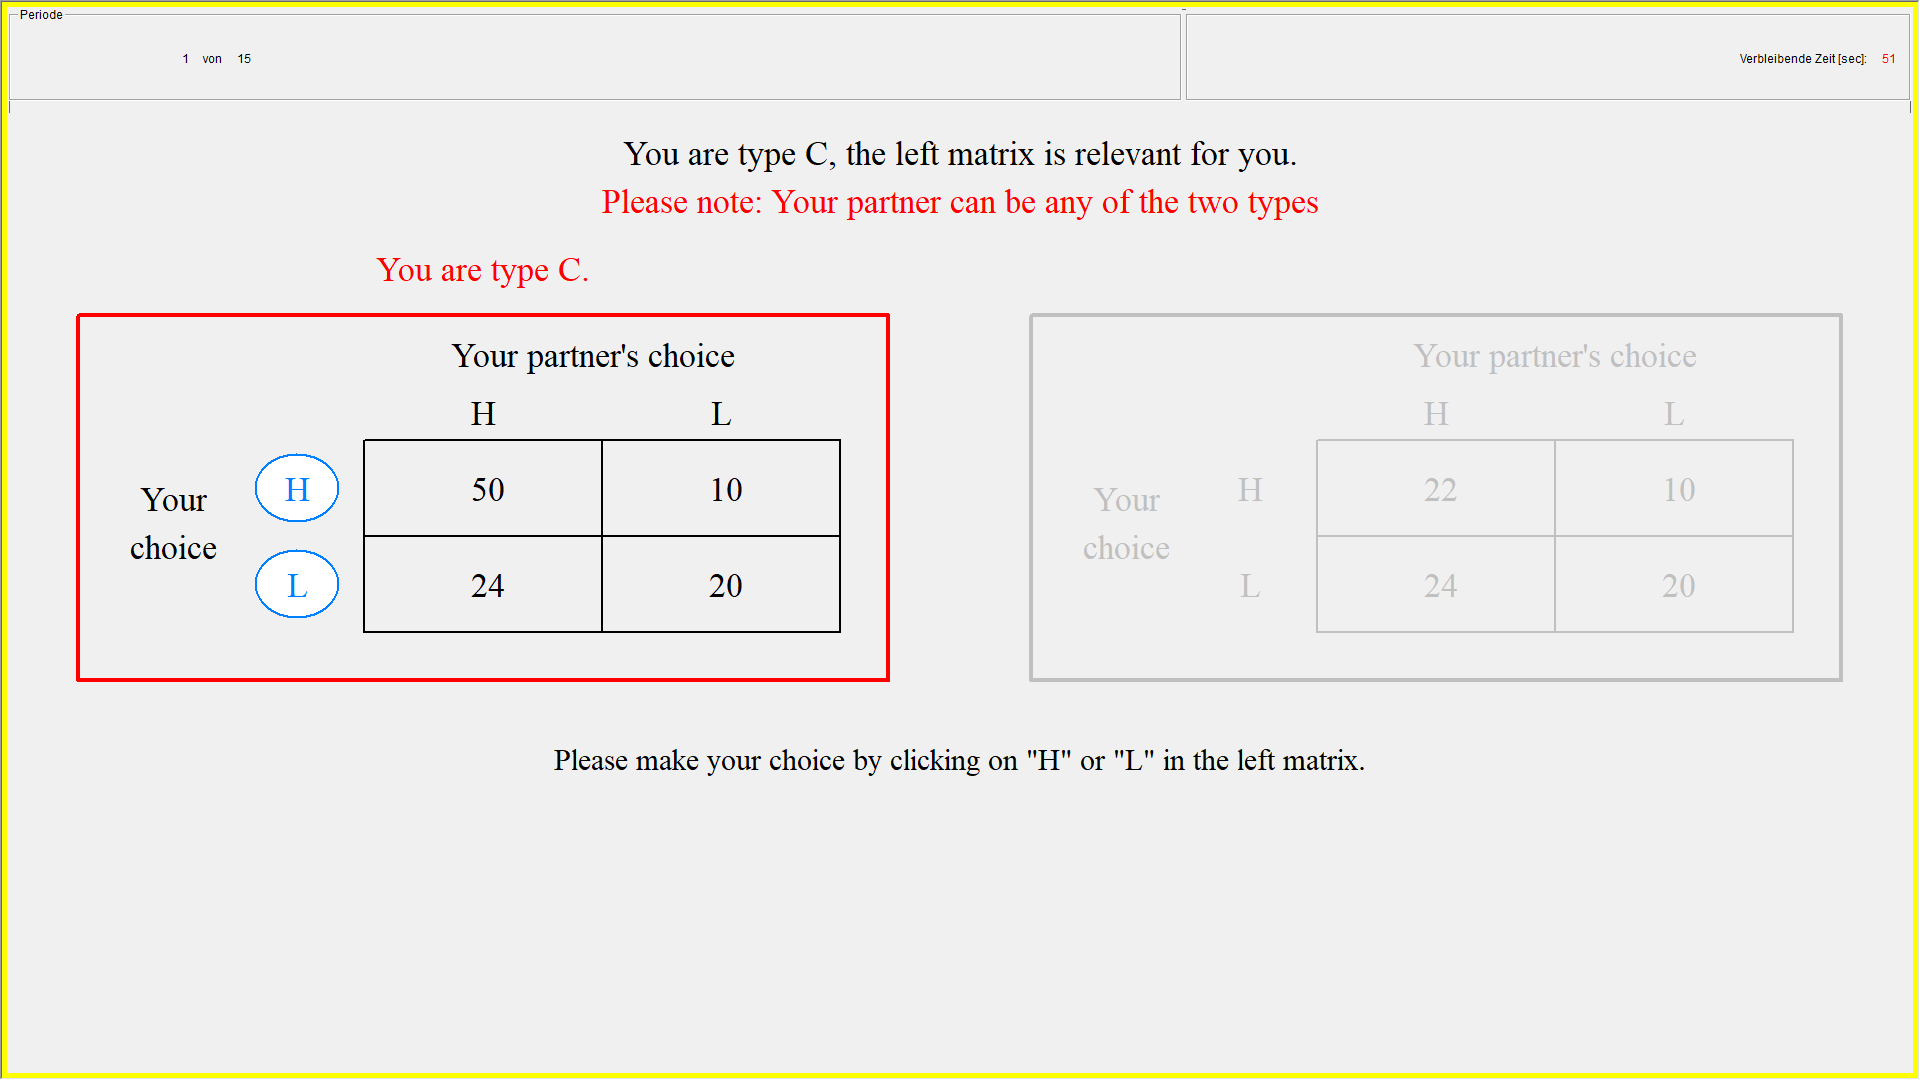
\includegraphics[width=1\textwidth]{fig1-NC-instructions.png}
  \label{fig:fig1-NC-instructions}
\end{figure}




You do not receive any information about the type of your partner, and your partner does not receive any information about your type. 

After your type and that of your partner have been randomly determined, you have to choose between two options, ``H'' and ``L", by clicking on the relevant blue button. When you are sure which choice to make, click on the blue button ``Confirm''.

 \begin{figure}[h]
   \centering
     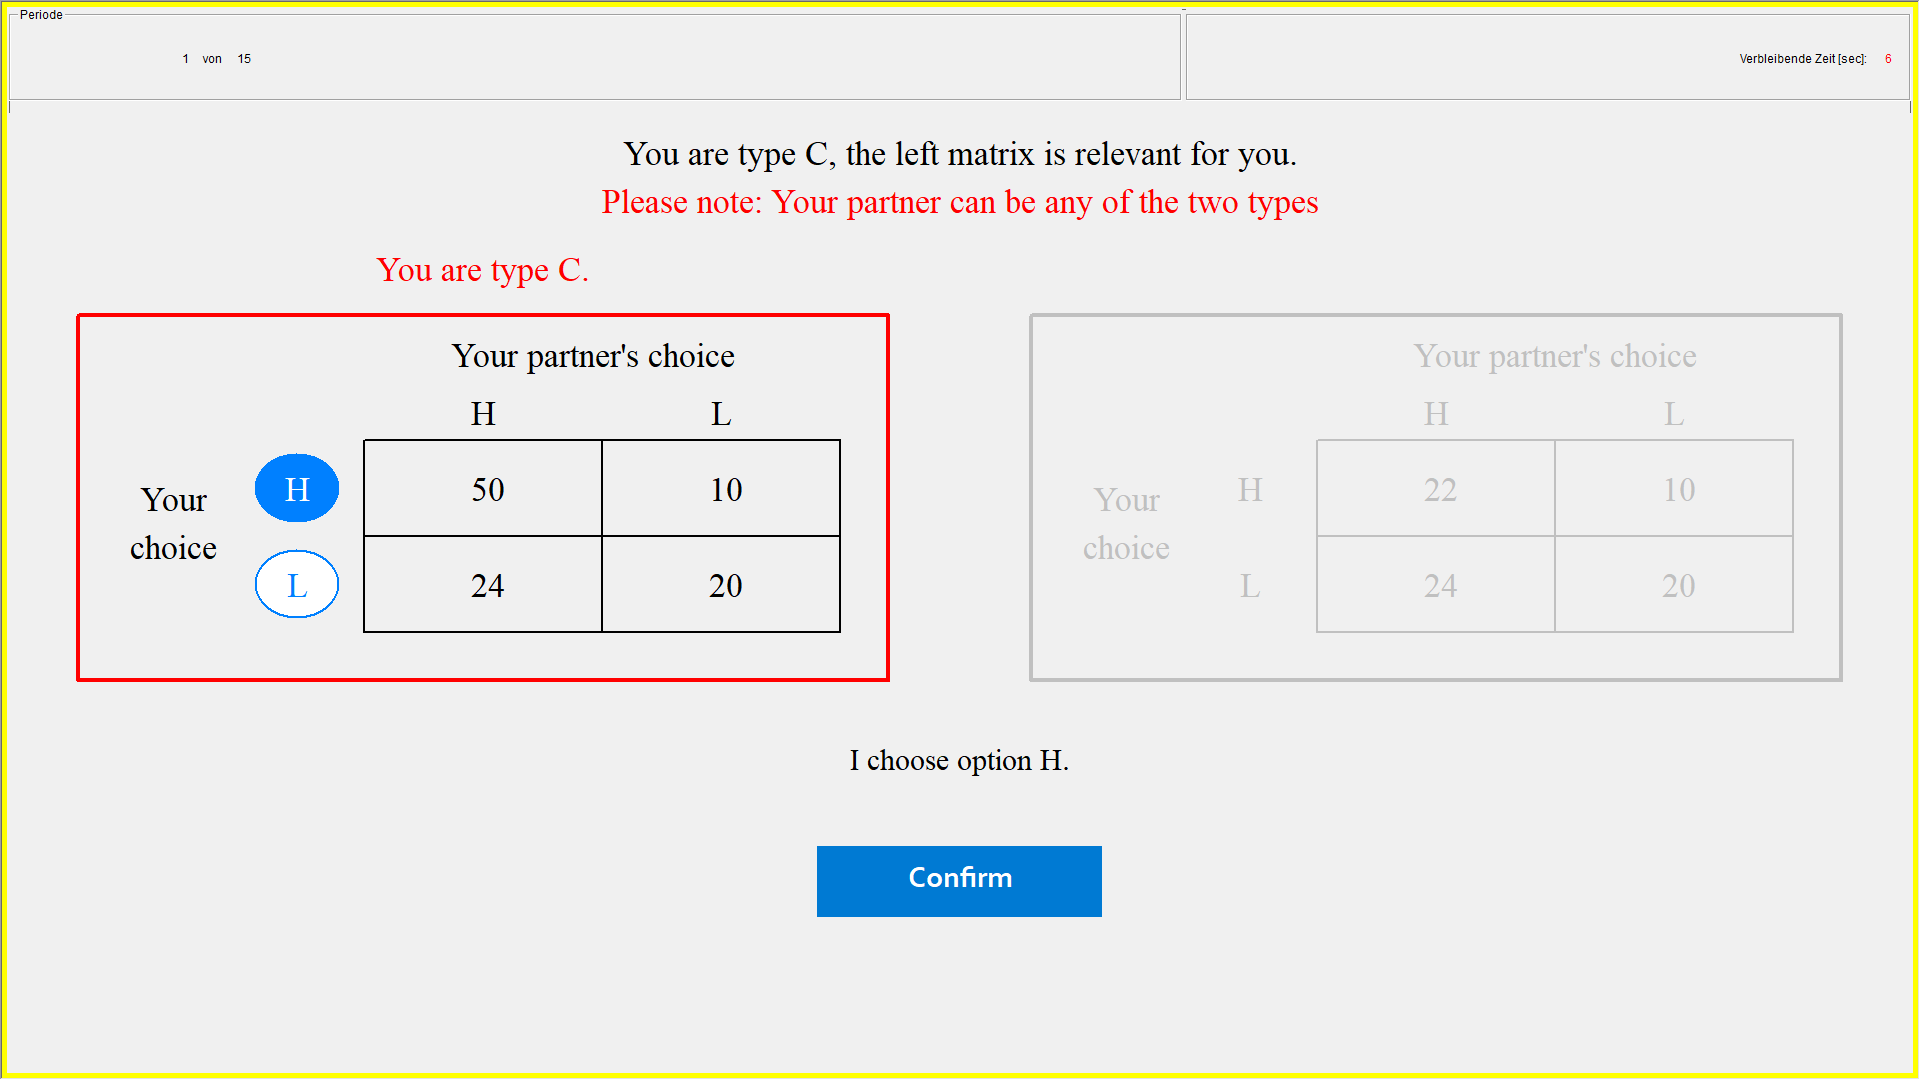
\includegraphics[width=.9\textwidth]{fig2-NC-instructions.png}
   \label{fig:fig2-NC-instructions}
 \end{figure}
 



You have at most one minute to decide which option to choose.

While you make your choice, your partner must also choose between ``H'' and ``L". You make your choice without knowing what your partner chooses, and your partner makes her/his choice without knowing your choice. 

After your decision and that of your partner the round ends, and your earnings for this round are calculated. As you can see from the screen-shot, your earning depends on your type, on your choice, and the choice of your partner. 

\textbf{Example}: You are of Type C, and therefore the left matrix is relevant for you. You choose H, and you partner chooses L. Therefore, your earnings are 10 ECUs in that round. Assume that your partner is of Type D in this round, i.e. the right matrix is relevant for her/him. In this case her/his earnings are 24. 

After the experiment ends, you will be asked to fill in a short questionnaire. After that you will be paid in private. Your overall earnings are the sum of the earnings you got in all 15 rounds. As already mentioned, the exchange rate between ECU and Euro is 25 ECU = 1 Euro. On top you will also get 4 Euros as a show up fee. The overall amount will appear on your screen, and paid to you in private by the experimenters. 

Do you have any questions? 




\textbf{Control Questionnaire}

The following questionnaire is anonymous and serves the sole purpose of verifying your understanding of this experiment. If you are uncertain about how to answer a questions, please consult the instructions or ask one of the experimenters.

Once you have finished the questionnaire, please raise your hand and an experimenter will come and check your answers.

1) You are of type D and you choose action L. Your partner is of type D and chooses action L.

What are your earnings in this round?
What are your partner’s earnings in this round?

2) You are of type C and choose action H. You partner is also of type C and chooses action H.

What are your earnings in this round?
What are your partner’s earnings in this round?


3) You are of type D and choose H. Your partner is of type C and chooses L.

What are your earnings in this round?
What are your partner’s earnings in this round?


\subsection{Instructions for the CT environment}

Welcome to the experiment on interactive decision-making, conducted by researchers from the Université libre de Bruxelles.

During this experiment you will earn an amount of money determined by your choices and by those of the other participants. All results will be analyzed anonymously, and your privacy is guaranteed. It is very important that you do not communicate with the other participants, neither verbally nor in any other way. If you have any question, please raise your hand and an experimenter will answer your question. If you communicate with the other participants during the experiment, you would have to leave the experiment without being paid. 

During the experiment your earnings are counted in Experimental Currency Units (ECUs). At the end of the experiment your earnings will be exchanged into Euros with an exchange rate of 1 Euro for 25 ECUs. You will be paid in cash immediately after the experiment. You will be paid privately, i.e. the other participants will not be informed about your earnings.

The whole experiment consists of 15 rounds. In each round you will be matched with a second participant, your ``partner". Your partner changes from round to round with your partner being determined randomly. It is possible that you might have the same partner during some rounds. But no participant gets any information about the identity of her/his partner. Therefore, it is impossible to identify the partner, and it is impossible to be identified by the partner.

Each round consists of 2 stages:

Stage 1: Your type and the type of your partner are determined. After being informed about your type (but not about the type of your partner), you decide whether you send a message to your partner or not. At the same time, your partner decides whether to send the a message to you or not.

Stage 2: You have to choose between two options, “H” or “L”. At the same time, your partner chooses between H and L. 

How much you earn in a certain round (your ``earnings") depends on your type, which option you choose, and which option your partner chooses. 

Detailed description of the two stages: 

\textbf{Stage 1}: At the beginning of each round your type is determined. You can be of two different types: Type “C” or Type “D”. If you are of Type C (as depicted on the screen-shot), the left earning matrix is relevant for your payment. If you are of Type D, the right earning matrix is relevant for you. 

\begin{figure}[h]
  \centering
    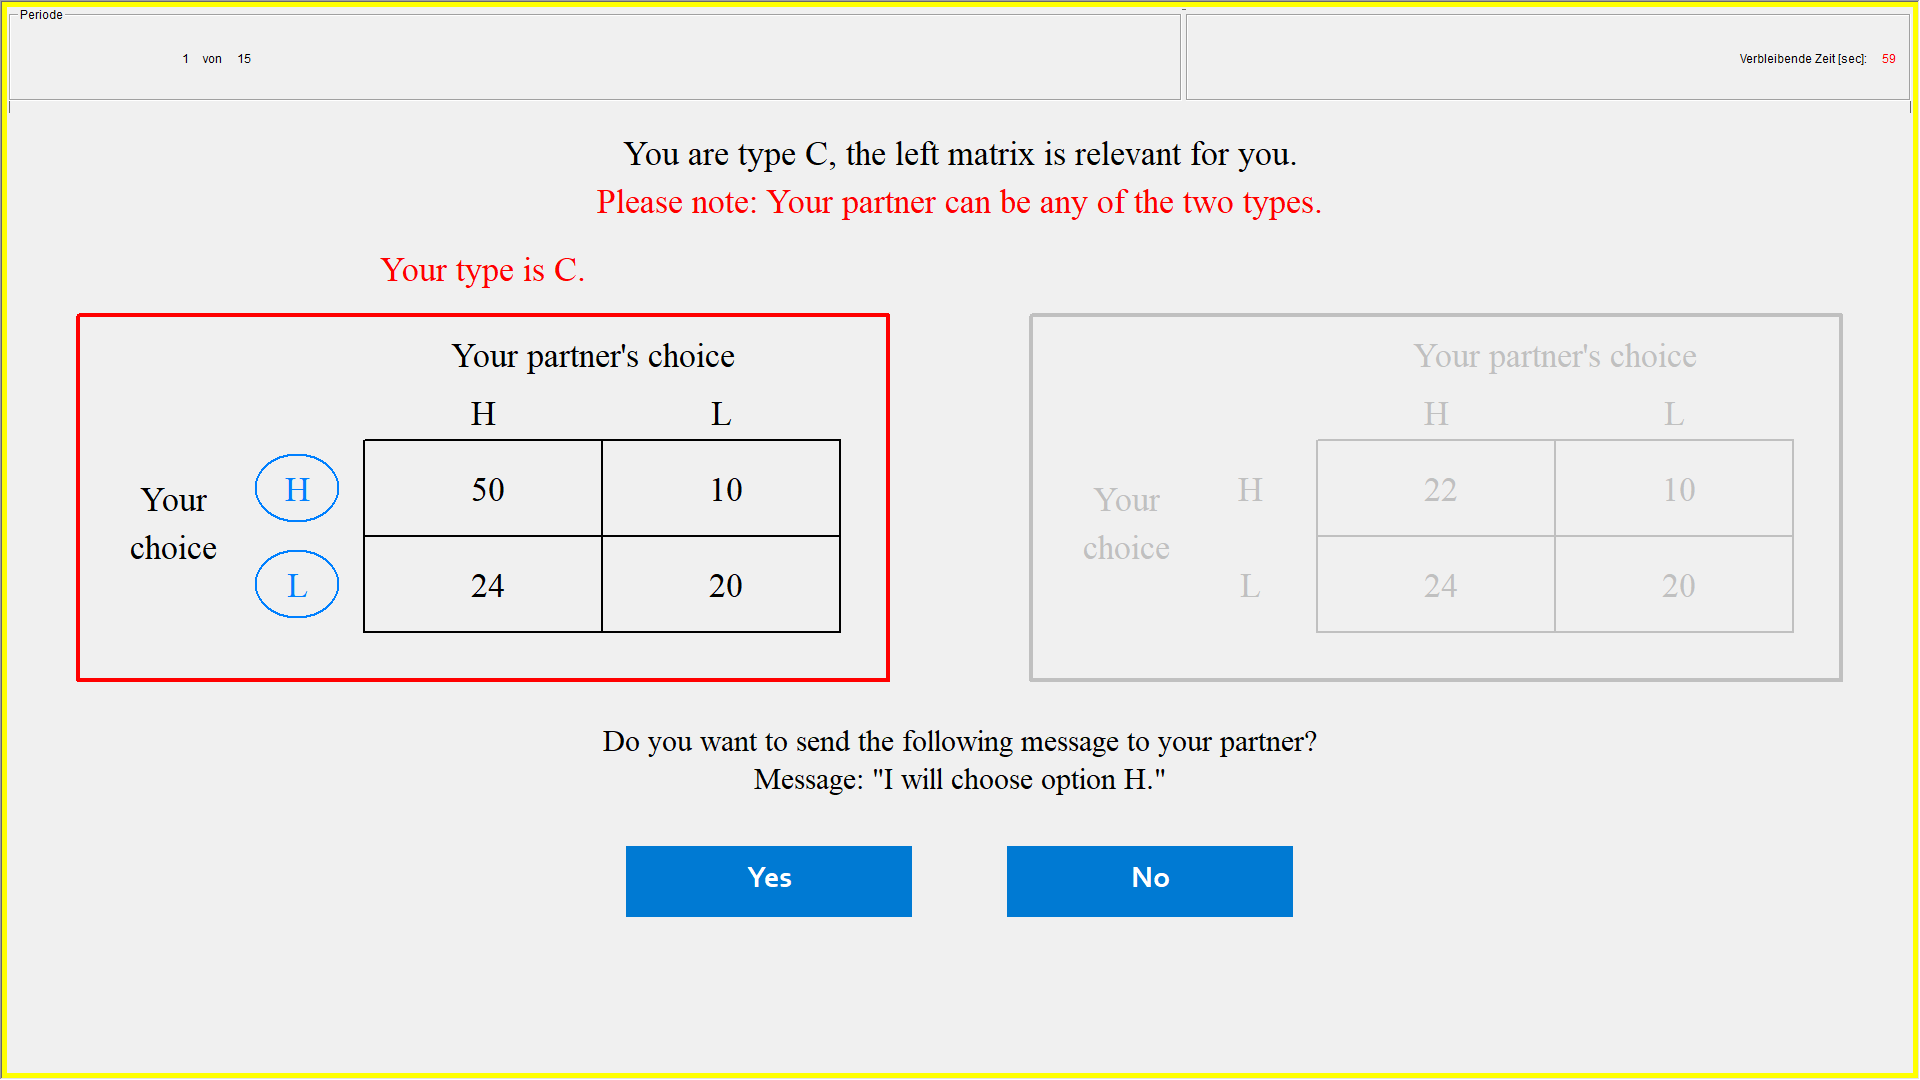
\includegraphics[width=.9\textwidth]{fig1-CT-instructions.png}
  \label{fig:fig1-CT-instructions}
\end{figure}


In every round your type will be determined randomly with equal probability ("fifty/fifty"). Similarly, the type of your partner is determined by the same random process. Your type and that of your partner might be the same, the types differ.
At the beginning of the round you will be informed about the type you are in this round. Your partner is also of the two possible types, but you will not be informed of which type he is. You only know that your partner is of Type C or Type D with equal probability.

Now you have to choose whether you want to send a message to your partner or not. The message refers to your choice in the Stage 2 and reads: “I will choose H” to your partner. If you want to send this message, click on the button ``Yes" on the screen below. If you do not want to send the message, click on the button ``No". 

You have at most one minute to decide whether you want to send the message or not. 

Note that the message is not binding for your actual choice in Stage 2 - if you send the message, you are nonetheless allowed to choose option ``L".

Your partner has to decide whether to send the same, non-binding message to you, too.

At the end of Stage 1, you get informed whether your partner sent you the message, and your partner gets informed whether you sent the message. 

\begin{figure}[h]
  \centering
    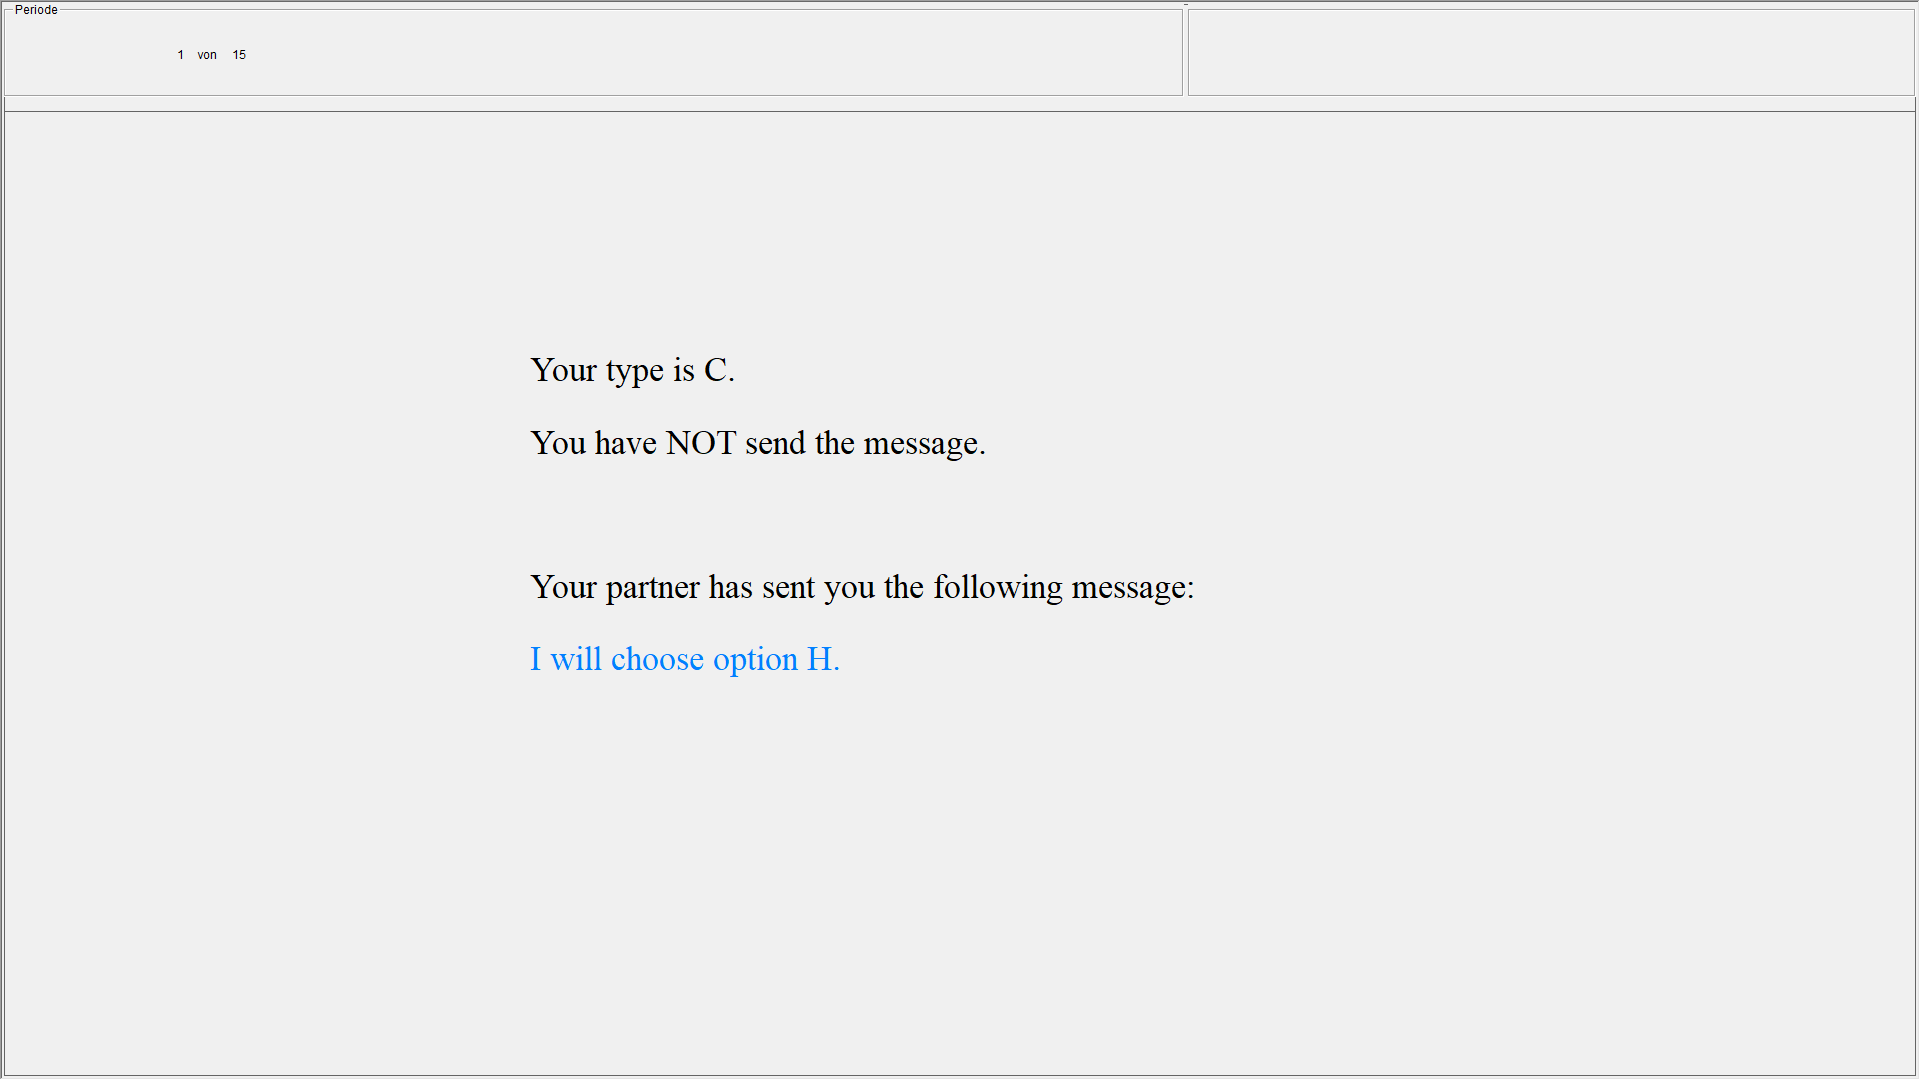
\includegraphics[width=.9\textwidth]{fig2-CT-instructions.png}
  \label{fig:fig2-CT-instructions}
\end{figure}


\textbf{Stage 2}: In stage 2 you have to choose between options, ``H'' and ``L", by clicking on the relevant blue button. 
If you are of Type C, the left matrix is relevant for you, if you are of type D, the right one.

When you are sure which choice to make, click on the blue button ``Confirm''.

\begin{figure}[h]
  \centering
    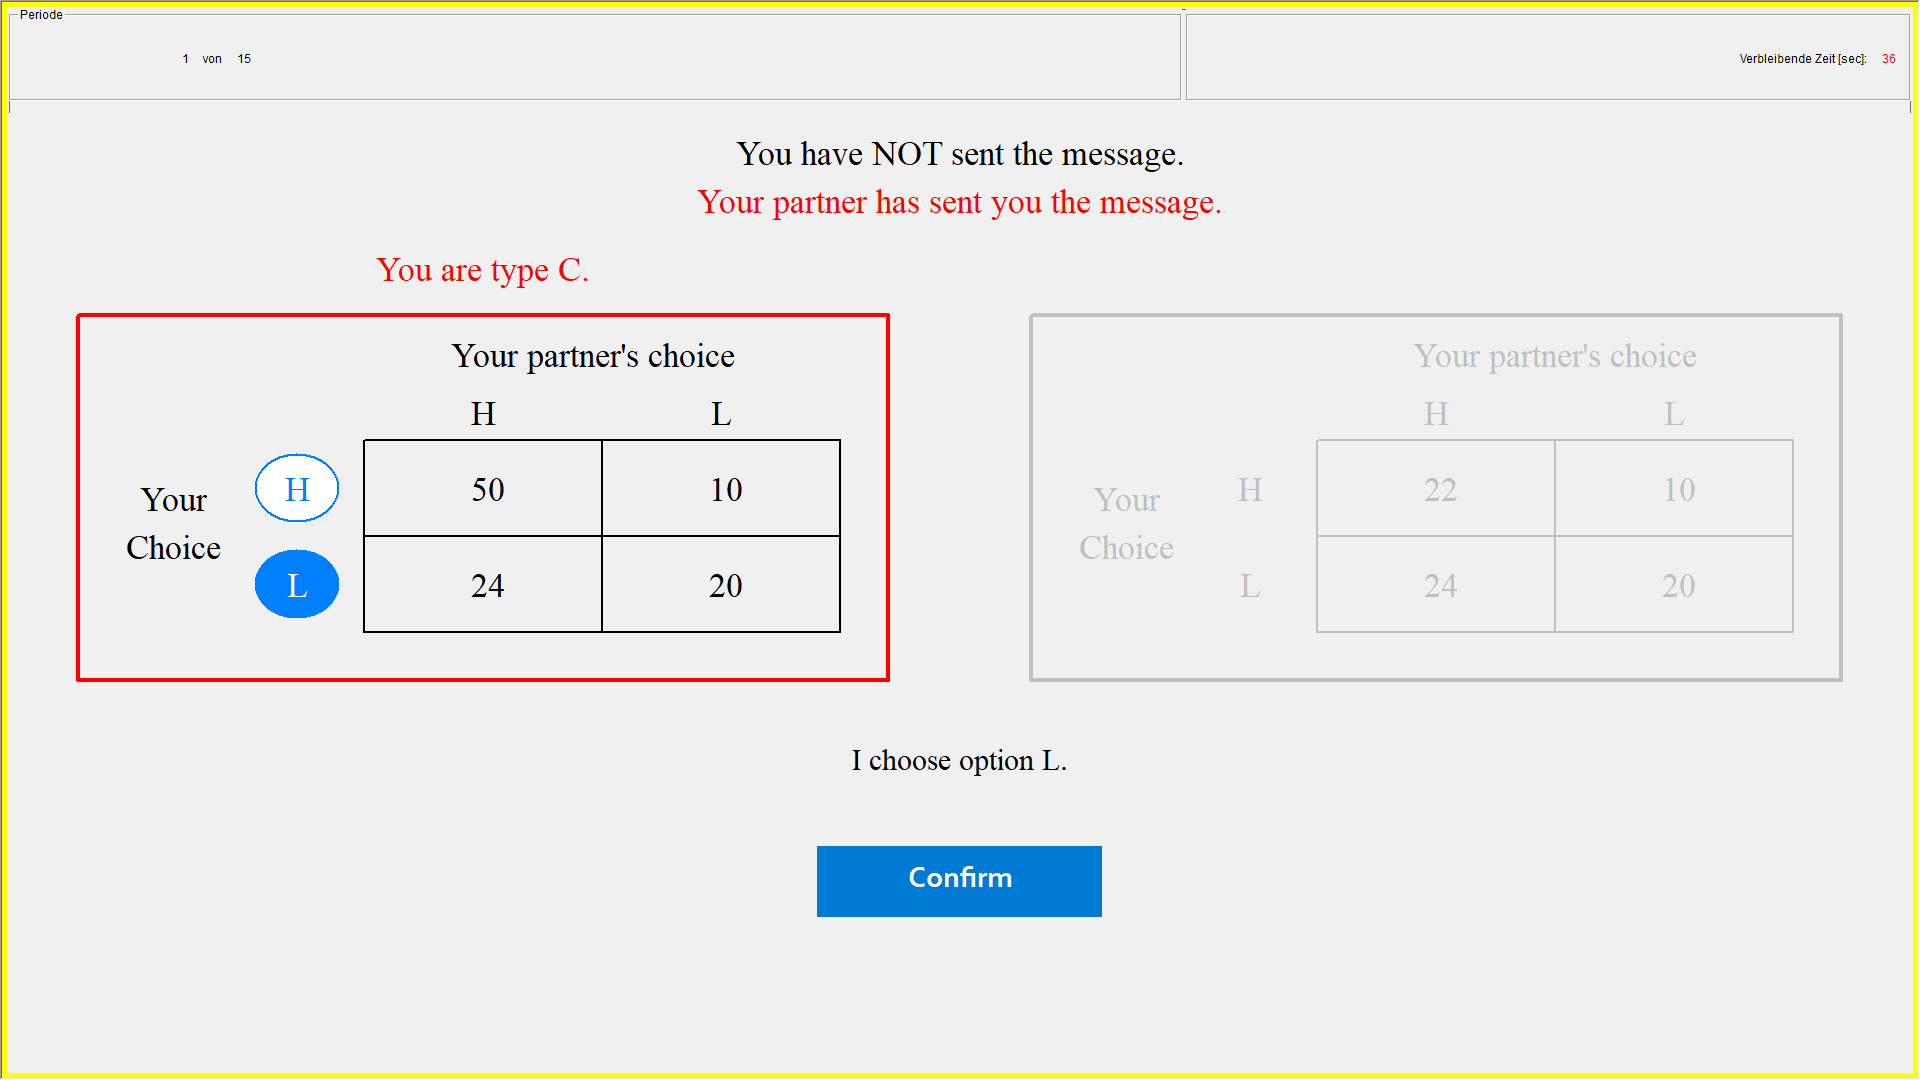
\includegraphics[width=.9\textwidth]{fig3-CT-instructions.png}
  \label{fig:fig3-CT-instructions}
\end{figure}

 
You have at most one minute to decide which option to choose.

While you make your choice, your partner must also choose between ``H'' and ``L". You make your choice without knowing what your partner chooses, and your partner makes her/his choice without knowing your choice. 

After the two stages the round ends, and your earnings for this round are calculated. As you can see from the screen-shot, your earning depends on your type, on your choice, and the choice of your partner. 

\textbf{Example}: You are of Type C, and therefore the left matrix is relevant for you. You choose H, and you partner chooses L. Therefore, your earnings are 10 ECUs in that round. Assume that your partner is of Type D in this round, i.e. the right matrix is relevant for her/him. In this case her/his earnings are 24. 

After the experiment ends, you will be asked to fill a short questionnaire. The sum of your earnings will be transformed into Euros with a change rate of 25 ECUs to 1 Euro. On top you will also get 4 Euros as a show up fee. The overall amount will appear on your screen, and paid to you in private by the experimenters. 

Do you have any questions? 

\textbf{Control Questionnaire}

Dear Participant,

the following questionnaire is anonymous and serves the sole purpose of verifying your understanding of this experiment. If you are uncertain about how to answer a questions, please consult the instructions or ask one of the experimenters.

Once you have finished the questionnaire, please raise your hand and an experimenter will come and check your answers.

1) You are of type D and you choose action L. Your partner is of type D and chooses action L.

What are your earnings in this round?
What are your partner’s earnings in this round?

2) You are of type C and choose action H. You partner is also of type C and chooses action H.

What are your earnings in this round?
What are your partner’s earnings in this round?


3) You are of type D and choose H. Your partner is of type C and chooses L.

What are your earnings in this round?
What are your partner’s earnings in this round?


\subsection{Instructions for the FC environment}

Welcome to the experiment on interactive decision-making, conducted by researchers from the Université libre de Bruxelles.

During this experiment you will earn an amount of money determined by your choices and by those of the other participants. All results will be analyzed anonymously, and your privacy is guaranteed. It is very important that you do not communicate with the other participants, neither verbally nor in any other way. If you have any question, please raise your hand and an experimenter will answer your question. If you communicate with the other participants during the experiment, you would have to leave the experiment without being paid. 

During the experiment your earnings are counted in Experimental Currency Units (ECUs). At the end of the experiment your earnings will be exchanged into Euros with an exchange rate of 1 Euro for 25 ECUs. You will be paid in cash immediately after the experiment. You will be paid privately, i.e. the other participants will not be informed about your earnings.

The whole experiment consists of 15 rounds. In each round you will be matched with a second participant, your ``partner". Your partner changes from round to round with your partner being determined randomly. It is possible that you might have the same partner during some rounds. But no participant gets any information about the identity of her/his partner. Therefore, it is impossible to identify the partner, and it is impossible to be identified by the partner.

Each round consists of 2 stages:

Stage 1: Your type and the type of your partner are determined. After being informed about your type (but not about the type of your partner), you decide whether you send a message to your partner or not. At the same time, your partner decides whether to send the a message to you or not.

Stage 2: You have to choose between two options, “H” or “L”. At the same time, your partner chooses between H and L. 

How much you earn in a certain round (your ``net-earnings") depends on your type, whether you send a message to your partner or not, which option you choose, and which option your partner chooses. 

Detailed description of the two stages: 

\textbf{Stage 1}: At the beginning of each round your type is determined. You can be of two different types: Type “C” or Type “D”. If you are of type C (as depicted on the screen-shot), the left earning matrix is relevant for your payment. If you are of Type D, the right earning matrix is relevant for you. 
 
\begin{figure}[h]
  \centering
    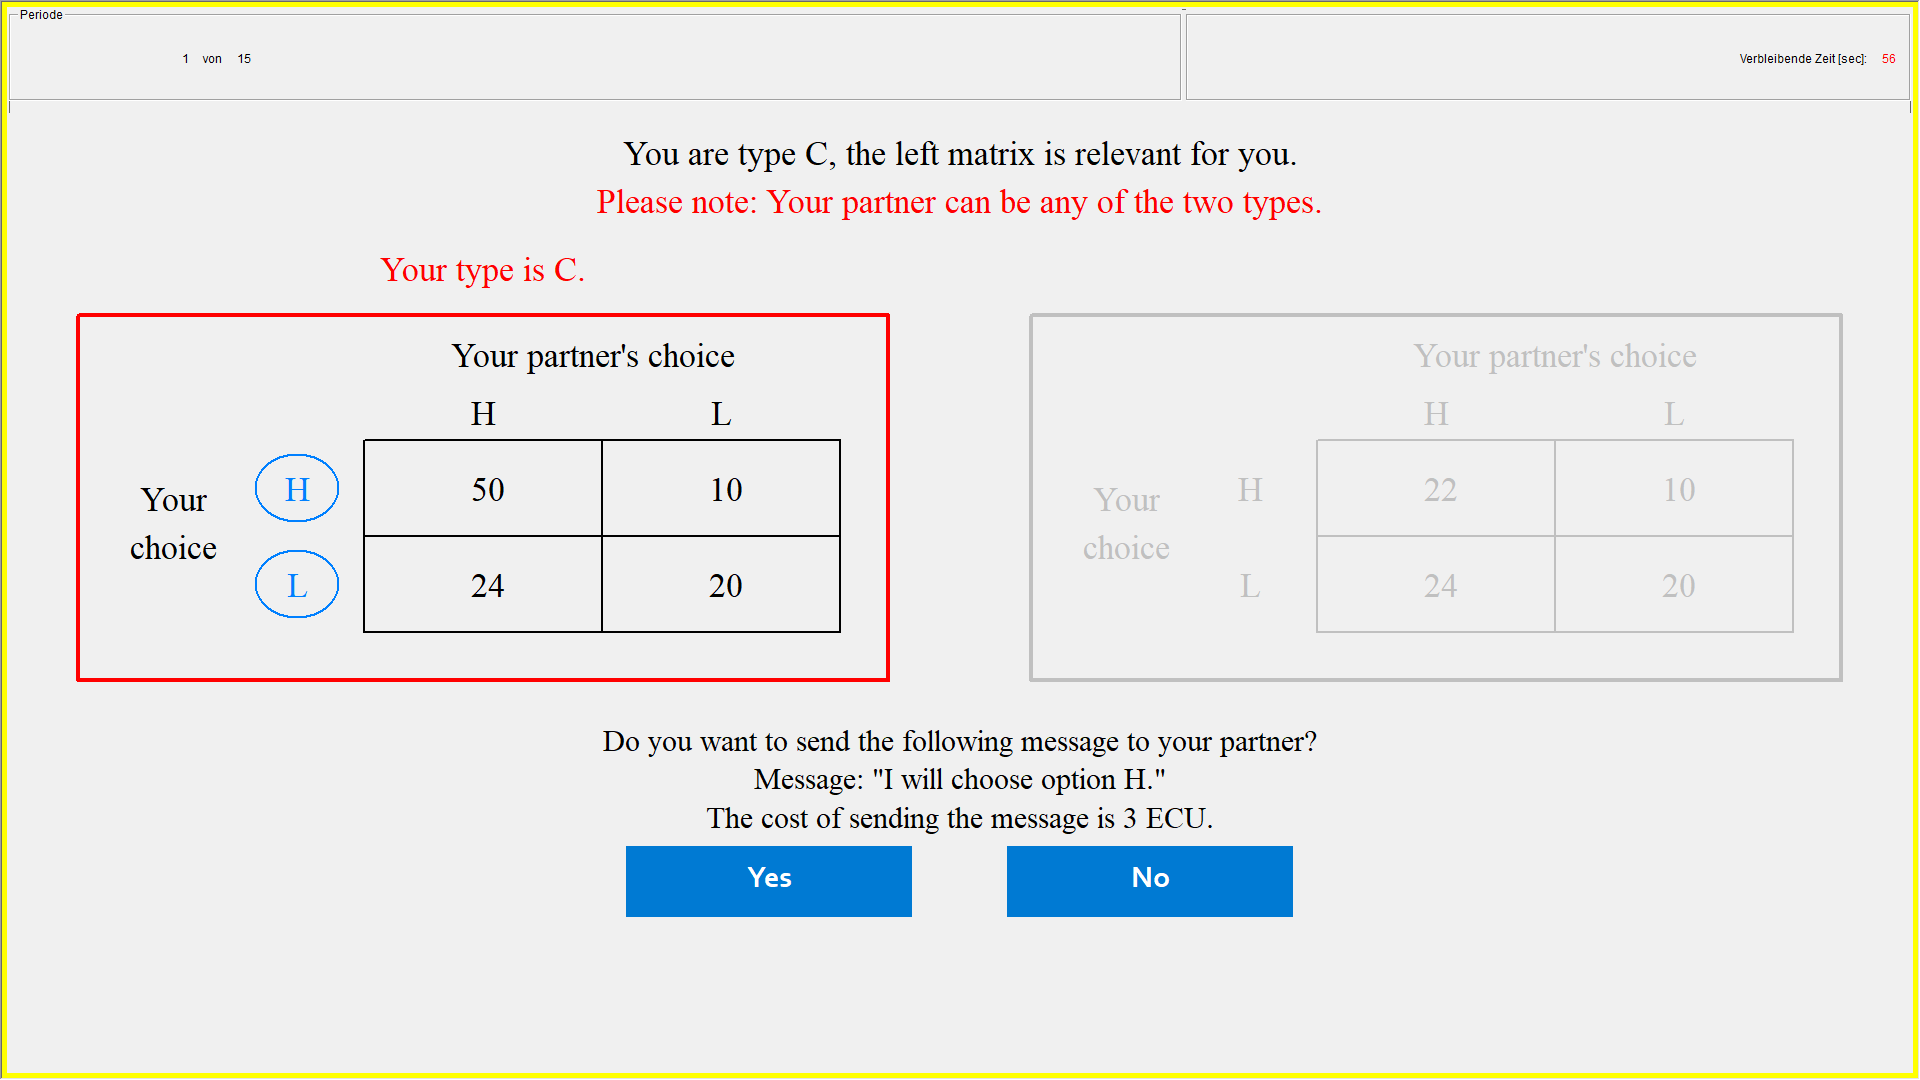
\includegraphics[width=.9\textwidth]{fig1-FC-instructions.png}
 \label{fig:fig1-FC-instructions}
\end{figure}

In every round your type will be determined randomly with equal probability ("fifty/fifty"). Similarly, the type of your partner is determined by the same random process. Your type and that of your partner might be the same, or the types differ.

At the beginning of the round you will be informed about the type you are in this round. Your partner is also of the two possible types, but you will not be informed of which type he is. You only know that your partner is of Type C or Type D with equal probability.

Now you have to choose whether you want to send a message to your partner or not. The message refers to your choice in the Stage 2 and reads: “I will choose H” to your partner. If you want to send this message, click on the button ``Yes'' on the screen below. If you do not want to send the message, click on the button ``No''. 

Sending the message costs you 3 ECUs, while sending no message costs you nothing.

You have at most one minute to decide whether you want to send the message or not. 

Note that the message is not binding for your actual choice in Stage 2 - if you send the message, you are nonetheless allowed to choose option ``L''.

Your partner has to decide whether to send the same, non-binding message to you, too.

At the end of Stage 1, you get informed whether your partner sent you the message, and your partner gets informed whether you sent the message. 

\begin{figure}[h]
  \centering
    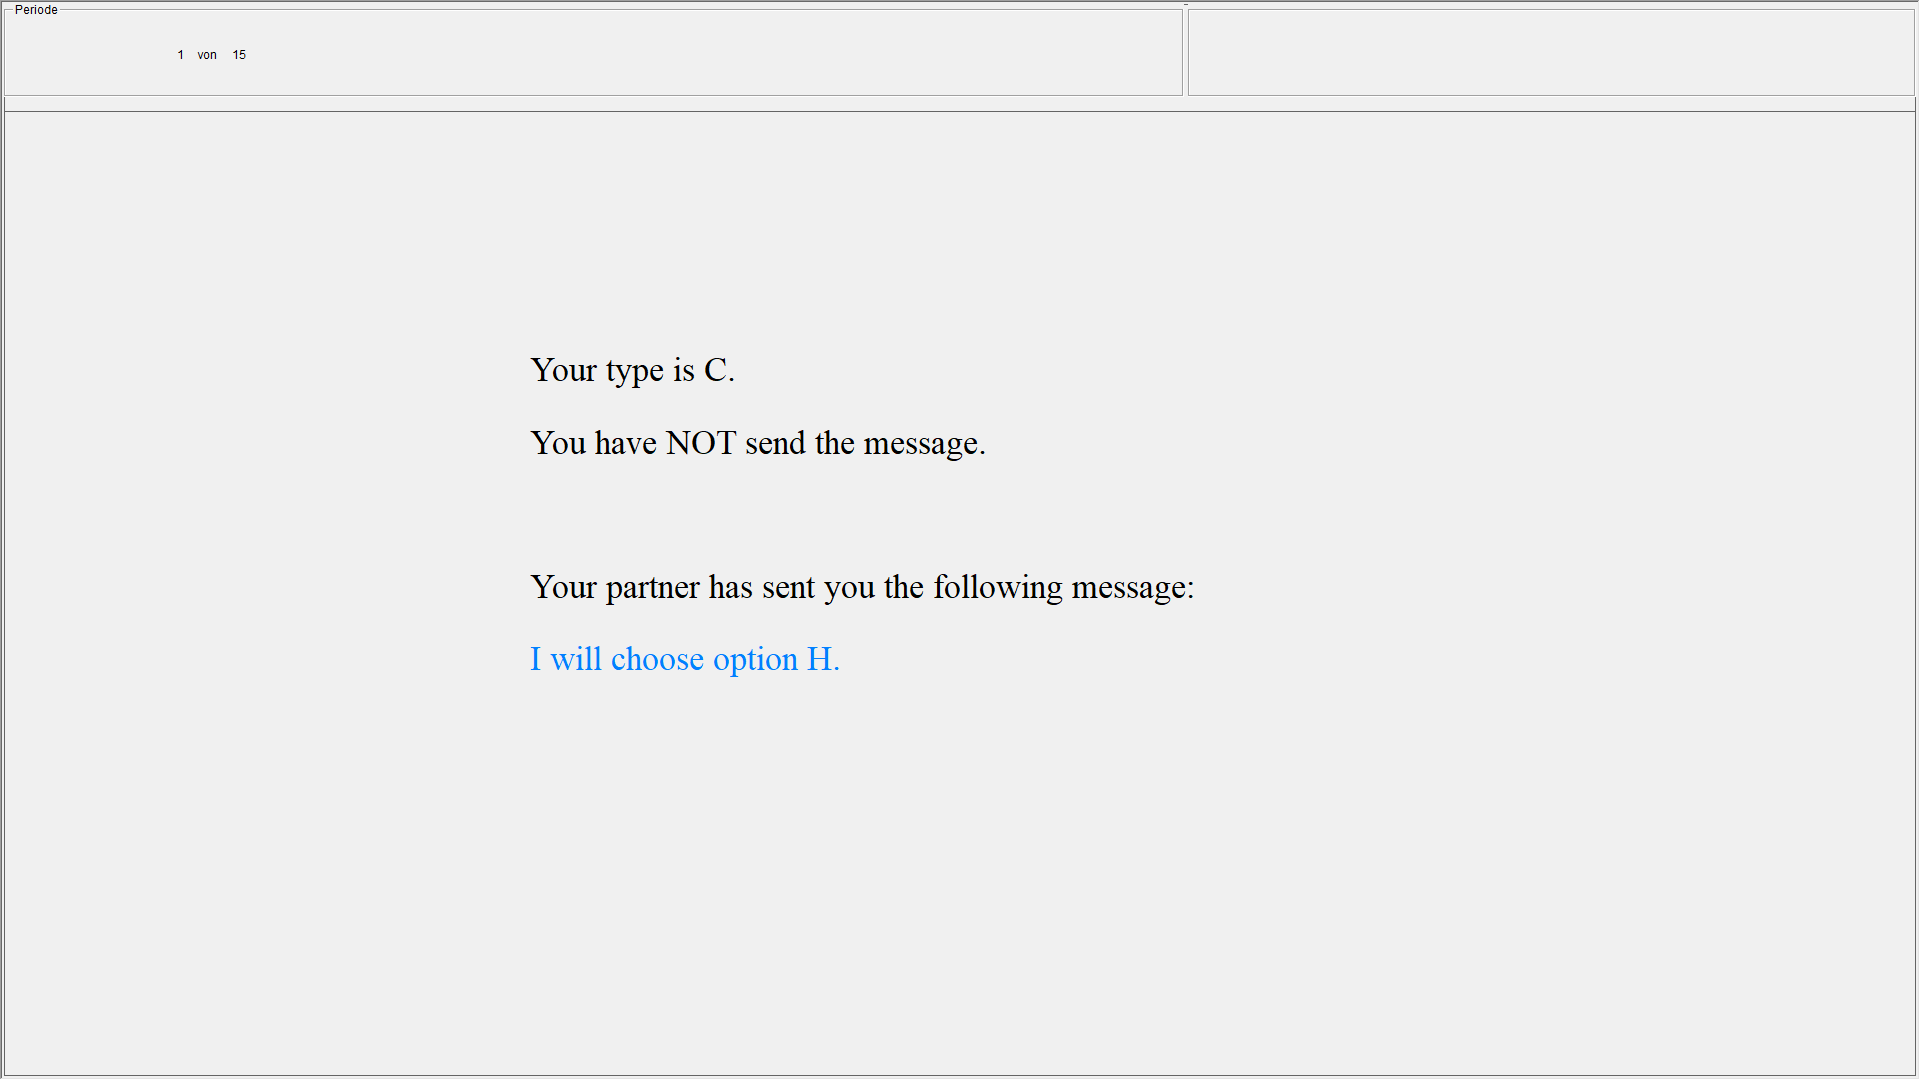
\includegraphics[width=.9\textwidth]{fig2-CT-instructions.png}
\label{fig:fig2-CT-instructions}
\end{figure}


\textbf{Stage 2}: In stage 2 you have to choose between options, ``H'' and ``L'', by clicking on the relevant blue button. 
If you are of Type C, the left matrix is relevant for you, if you are of type D, the right one.

When you are sure which choice to make, click on the blue button ``Confirm''.

 \begin{figure}[h]
   \centering
     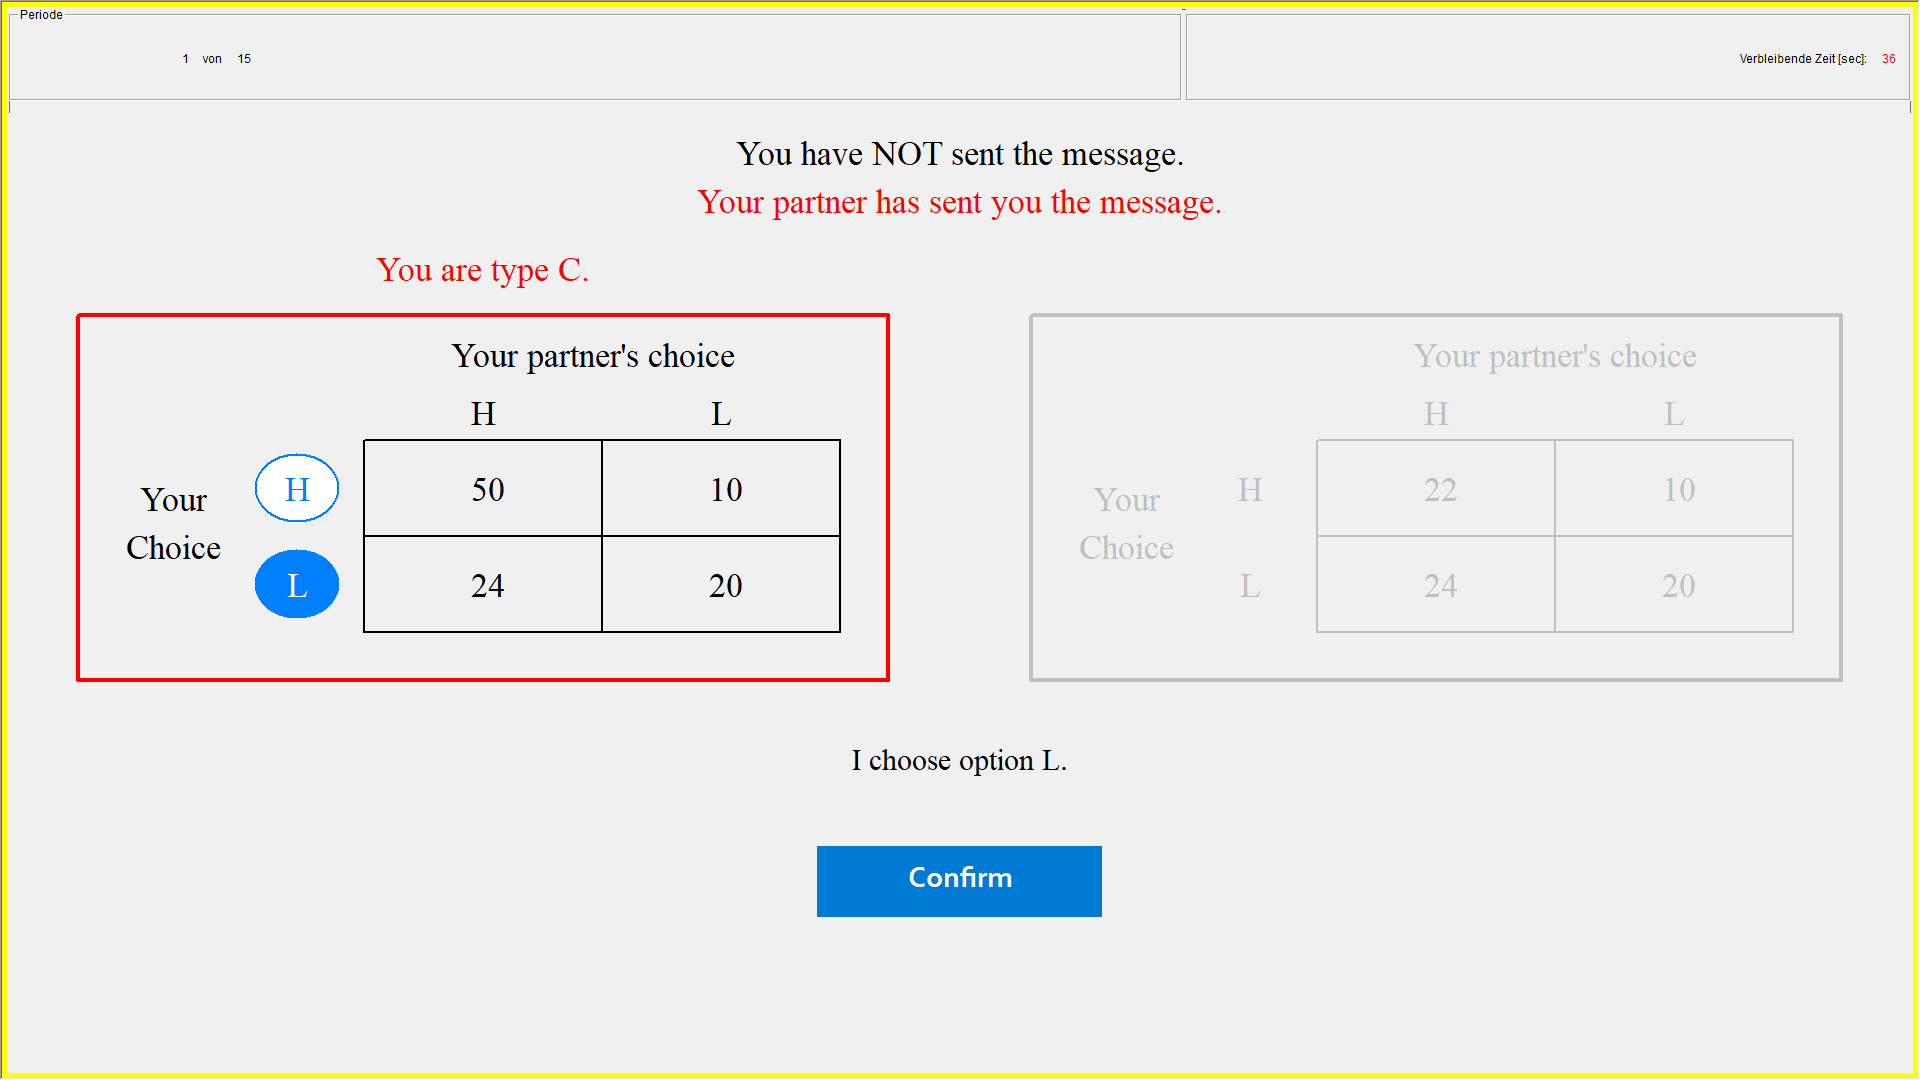
\includegraphics[width=.9\textwidth]{fig3-FC-instructions.png}
   \label{fig:fig3-FC-instructions}
 \end{figure}
 

You have at most one minute to decide.

While you make your choice, your partner must also choose between ``H'' and ``L". You make your choice without knowing what your partner chooses, and your partner makes her/his choice without knowing your choice. 

After the two stages the round ends, and your net-earnings for this round are calculated. As you can see from the screen-shot, your net-earnings depend on your type, whether you send a message to your partner or not, which option you choose, and which option your partner chooses. 

\textbf{Example}: You are of Type C, and therefore the left matrix is relevant for you. You send the message and this costs you three ECUs. You choose H, and you partner chooses L. Therefore, your earnings are 10-3= 7 ECUs in that round. Assume that your partner is of Type D in this round, i.e. the right matrix is relevant for her/him, and (s)he does not send a message. In this case her/his earnings are 24. 

After the experiment ends, you will be asked to fill a short questionnaire. The sum of your earnings will be transformed into Euros with a change rate of 25 ECUs to 1 Euro. On top you will also get 4 Euros as a show up fee. The overall amount will appear on your screen, and paid to you in private by the experimenters. 

Do you have any questions? 

\textbf{Control Questionnaire}

The following questionnaire is anonymous and serves the sole purpose of verifying your understanding of this experiment. If you are uncertain about how to answer a questions, please consult the instructions or ask one of the experimenters.

Once you have finished the questionnaire, please raise your hand and an experimenter will come and check your answers.

1) You are of type D, you send the message, and you choose action L. Your partner is of type 2, (s)he does not send the message, and chooses action L.

What are your earnings in this round?
What are your partner’s earnings in this round?

2) You are of type C, you do not send the message, and you choose action H. Your partner is of type C, (s)he sends the message, and chooses action H.

What are your earnings in this round?
What are your partner’s earnings in this round?


3) You are of type D, you do not send the message, and you choose action H. Your partner is of type C, (s)he does not send the message, and chooses action L.

What are your earnings in this round?
What are your partner’s earnings in this round?








\bibliographystyle{agsm}
\bibliography{collusion}
\end{document}